%%%%%%%%%%%%%%%%%%%%%%%%%%%%%%%%%%%%%%
%%%%%%%%%%%%%%%%%%%%%%%%%%%%%%%%%%%%%%
% Do not edit the TeX file your work
% will be overwritten.  Edit the RnW
% file instead.
%%%%%%%%%%%%%%%%%%%%%%%%%%%%%%%%%%%%%%
%%%%%%%%%%%%%%%%%%%%%%%%%%%%%%%%%%%%%%





\newcommand{\DefineMacros}{
\newcommand{\AlexanderNSur}{4,364}
\newcommand{\AlexanderNTar}{64,784,329}
\newcommand{\AlexanderYbar}{0.462}
\newcommand{\AlexanderMrpMu}{0.288}
\newcommand{\AlexanderRakingMu}{0.263}
\newcommand{\AlexanderNumBoots}{100}
\newcommand{\AlexanderMCMCTimeMins}{95}
\newcommand{\AlexanderMrplewTimeSecs}{664}
\newcommand{\AlexanderMrPSd}{1.06}
\newcommand{\AlexanderRakingSd}{1.39}
\newcommand{\AlexanderMrPPostSd}{1.09}
\newcommand{\StoriesNSur}{4,803}
\newcommand{\StoriesNTar}{406,886}
\newcommand{\StoriesYbar}{0.539}
\newcommand{\StoriesMrpMu}{0.522}
\newcommand{\StoriesRakingMu}{0.522}
\newcommand{\StoriesNumBoots}{100}
\newcommand{\StoriesMCMCTimeMins}{15}
\newcommand{\StoriesMrplewTimeSecs}{5}
\newcommand{\StoriesMrPSd}{0.523}
\newcommand{\StoriesRakingSd}{0.523}
\newcommand{\StoriesMrPPostSd}{0.527}
\newcommand{\LaxNSur}{6,341}
\newcommand{\LaxNTar}{994,486}
\newcommand{\LaxYbar}{0.333}
\newcommand{\LaxMrpMu}{0.457}
\newcommand{\LaxRakingMu}{0.345}
\newcommand{\LaxNumBoots}{100}
\newcommand{\LaxMCMCTimeMins}{39}
\newcommand{\LaxMrplewTimeSecs}{7}
\newcommand{\LaxMrPSd}{1.27}
\newcommand{\LaxRakingSd}{0.583}
\newcommand{\LaxMrPPostSd}{3.07}
\newcommand{\AlexanderColpert}{\texttt{\detokenize{decade_married_rk2009+:educ_group>BA}}}
\newcommand{\AlexanderPctflipped}{2}
\newcommand{\AlexanderShrink}{0}
\newcommand{\LaxColpert}{\texttt{\detokenize{edu.cat2}}}
\newcommand{\LaxPctflipped}{10}
\newcommand{\LaxShrink}{0}

}




%%%%%%%%%%%%%%%%%%%%%%%


\newcommand{\YpathPlot}{

\begin{knitrout}
\definecolor{shadecolor}{rgb}{0.969, 0.969, 0.969}\color{fgcolor}

{\centering 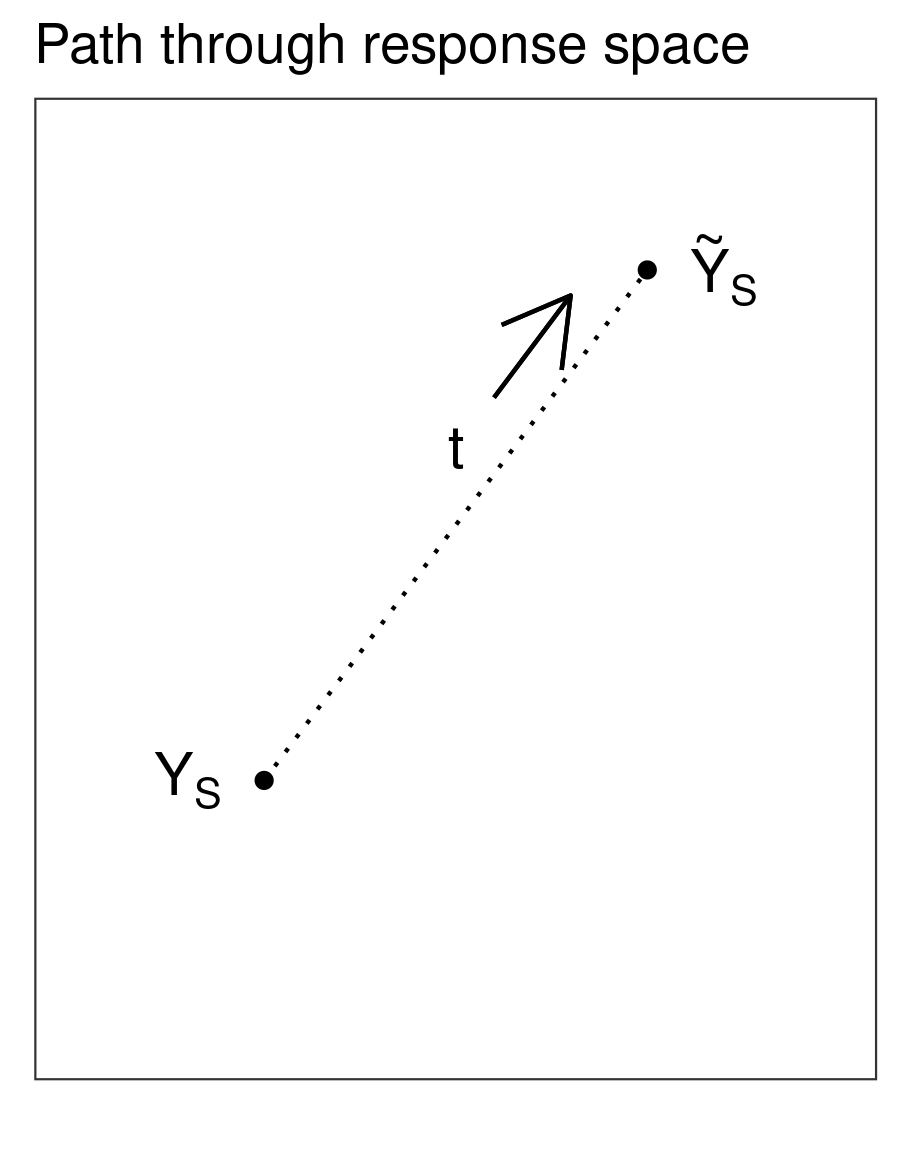
\includegraphics[width=0.98\linewidth,height=1.274\linewidth]{figure/ypath-1} 

}


\end{knitrout}

}


\newcommand{\YpathRegionPlot}{

\begin{knitrout}
\definecolor{shadecolor}{rgb}{0.969, 0.969, 0.969}\color{fgcolor}

{\centering 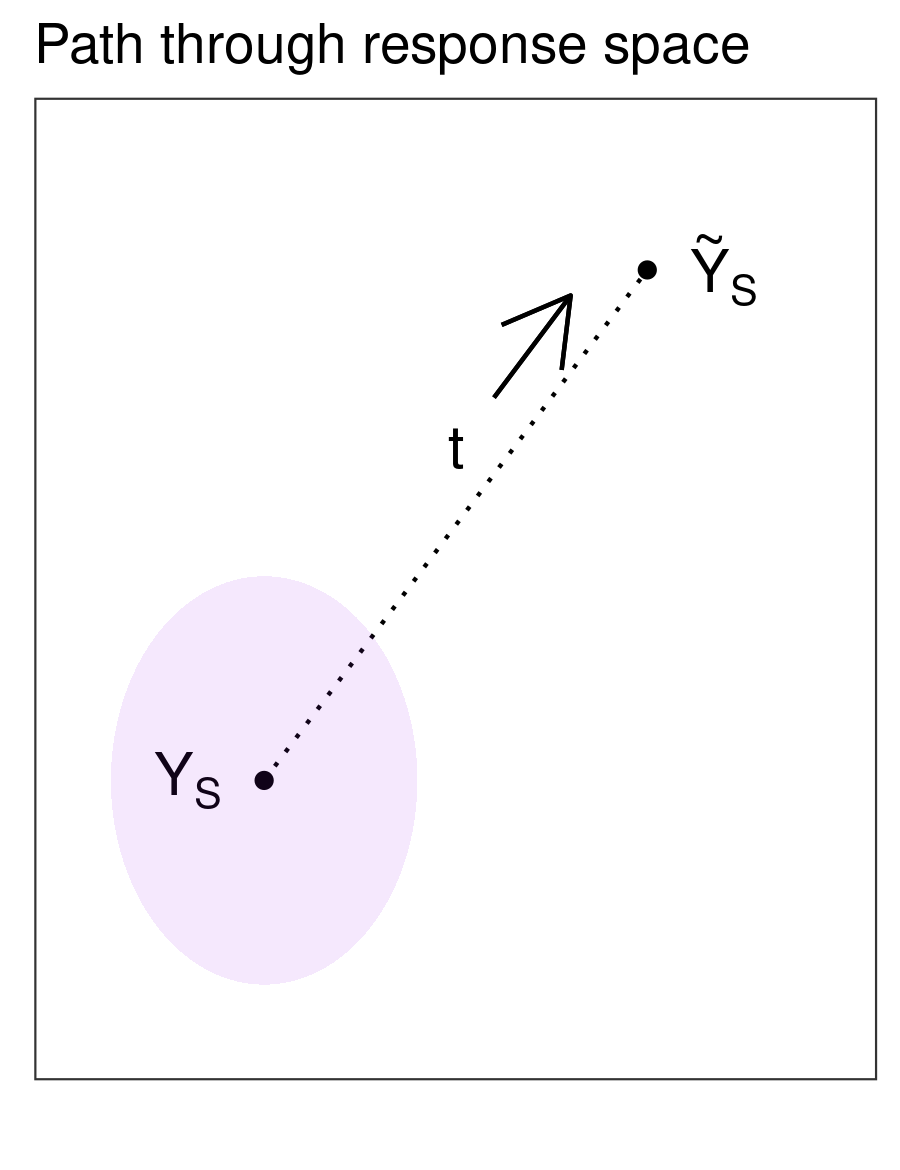
\includegraphics[width=0.98\linewidth,height=1.274\linewidth]{figure/ypathregion-1} 

}


\end{knitrout}

}




\newcommand{\CWPathPlot}{

\begin{knitrout}
\definecolor{shadecolor}{rgb}{0.969, 0.969, 0.969}\color{fgcolor}

{\centering 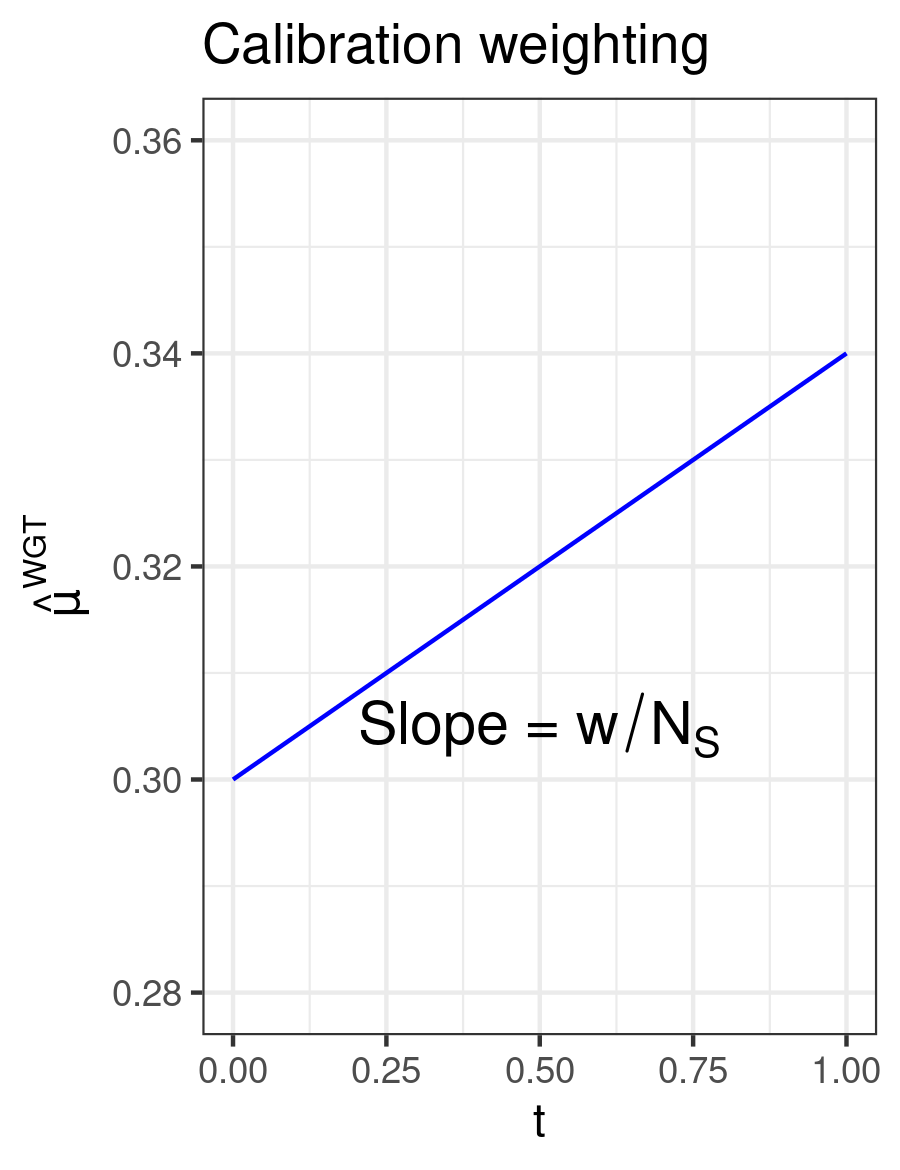
\includegraphics[width=0.98\linewidth,height=1.274\linewidth]{figure/cwpath-1} 

}


\end{knitrout}

}


\newcommand{\MrPPathPlot}{

\begin{knitrout}
\definecolor{shadecolor}{rgb}{0.969, 0.969, 0.969}\color{fgcolor}

{\centering 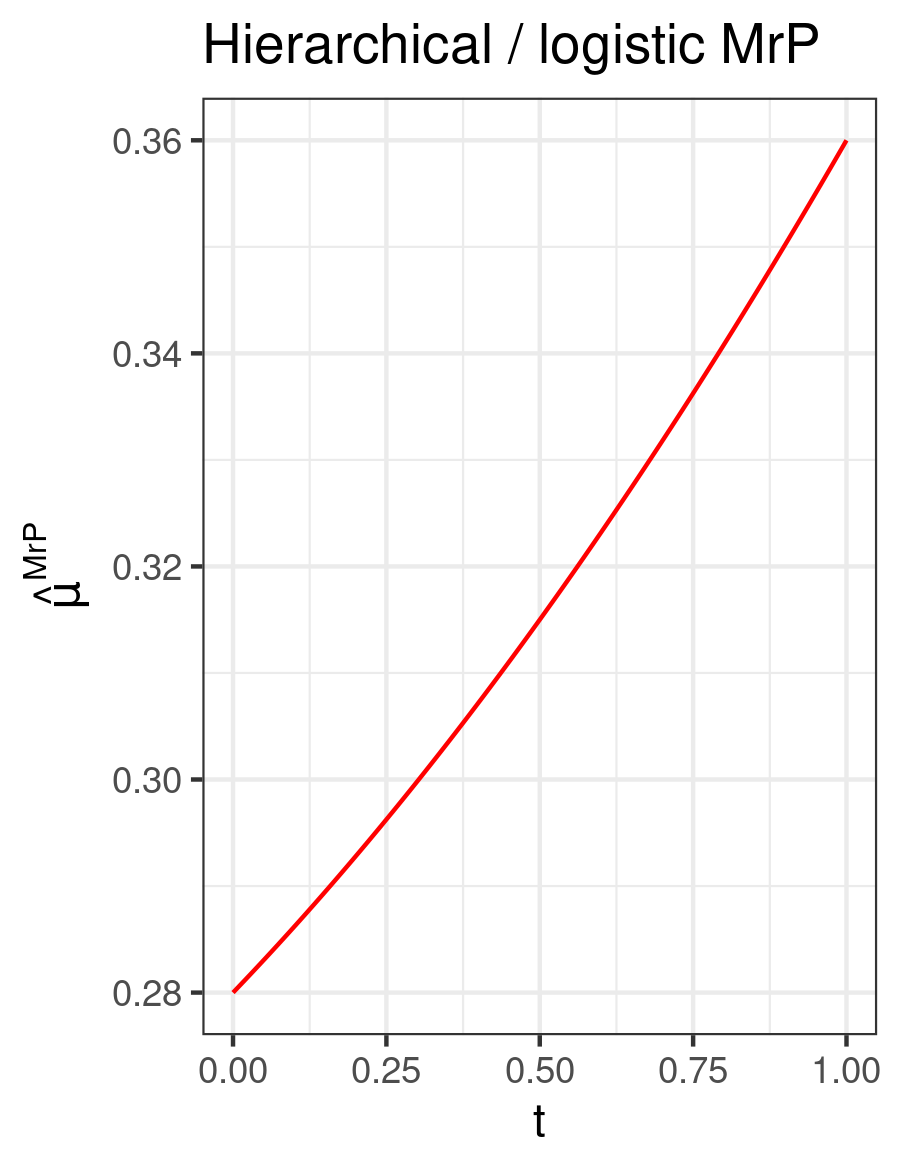
\includegraphics[width=0.98\linewidth,height=1.274\linewidth]{figure/mrppath-1} 

}


\end{knitrout}

}



\newcommand{\MrPlewPathPlot}{

\begin{knitrout}
\definecolor{shadecolor}{rgb}{0.969, 0.969, 0.969}\color{fgcolor}

{\centering 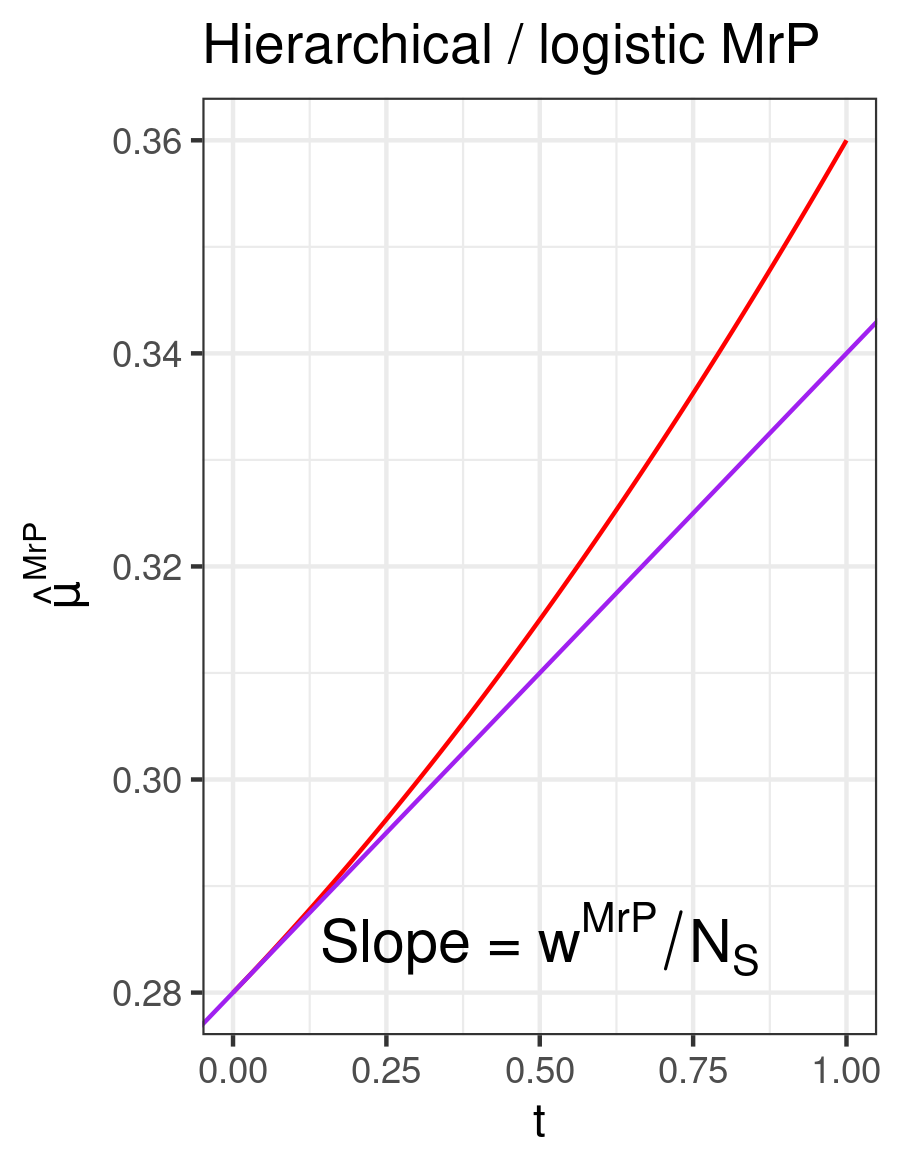
\includegraphics[width=0.98\linewidth,height=1.274\linewidth]{figure/mrplewpath-1} 

}


\end{knitrout}

}




%%%%%%%%%%%%%%%%%%%%%%%

\newcommand{\IntroPlot}{

\begin{knitrout}
\definecolor{shadecolor}{rgb}{0.969, 0.969, 0.969}\color{fgcolor}\begin{kframe}


{\ttfamily\noindent\bfseries\color{errorcolor}{\#\# Error in file(filename, "{}r"{}, encoding = encoding): cannot open the connection}}\end{kframe}
\end{knitrout}
}



% %%%%%%%%%%%%%%%%%%%%%%

\newcommand{\ExperimentTable}{
\begin{tabular}{lccc}
\hline
 & Name Change & Same-Sex Marriage & Election Forecasting \\
\hline
$\nsur$ & $\AlexanderNSur{}$ & $\LaxNSur{}$ & $\StoriesNSur{}$ \\
$\overline{\y}$ & $\AlexanderYbar{}$ & $\LaxYbar{}$ & $\StoriesYbar{}$ \\
$\muhat[\mrp]$ & $\AlexanderMrpMu{}$ & $\LaxMrpMu{}$ & $\StoriesMrpMu{}$ \\
$\muhat[\cal]$ & $\AlexanderRakingMu{}$ & $\LaxRakingMu{}$ & $\StoriesRakingMu{}$ \\
\hline
\end{tabular}

}


\newcommand{\AlexanderResidualTable}{
\begin{table}[!h]
\centering
\caption{\label{tab:alexanderresidtable}Mean response and residuals by interaction value for Name Change}
\centering
\begin{tabular}[t]{|r||l||l|}
\hline
\AlexanderColpert{} & $\overline{y}$ & $\overline{y - \hat{y}}$\\
\hline
0 & 0.412 & -0.001\\
\hline
1 & 0.560 & 0.002\\
\hline
\end{tabular}
\end{table}

}


% %%%%%%%%%%%%%%%%%%%%%%


% fig.scap prevents math in the caption optional argument
\newcommand{\VariancePlot}{

\begin{knitrout}
\definecolor{shadecolor}{rgb}{0.969, 0.969, 0.969}\color{fgcolor}\begin{figure}[H]

{\centering 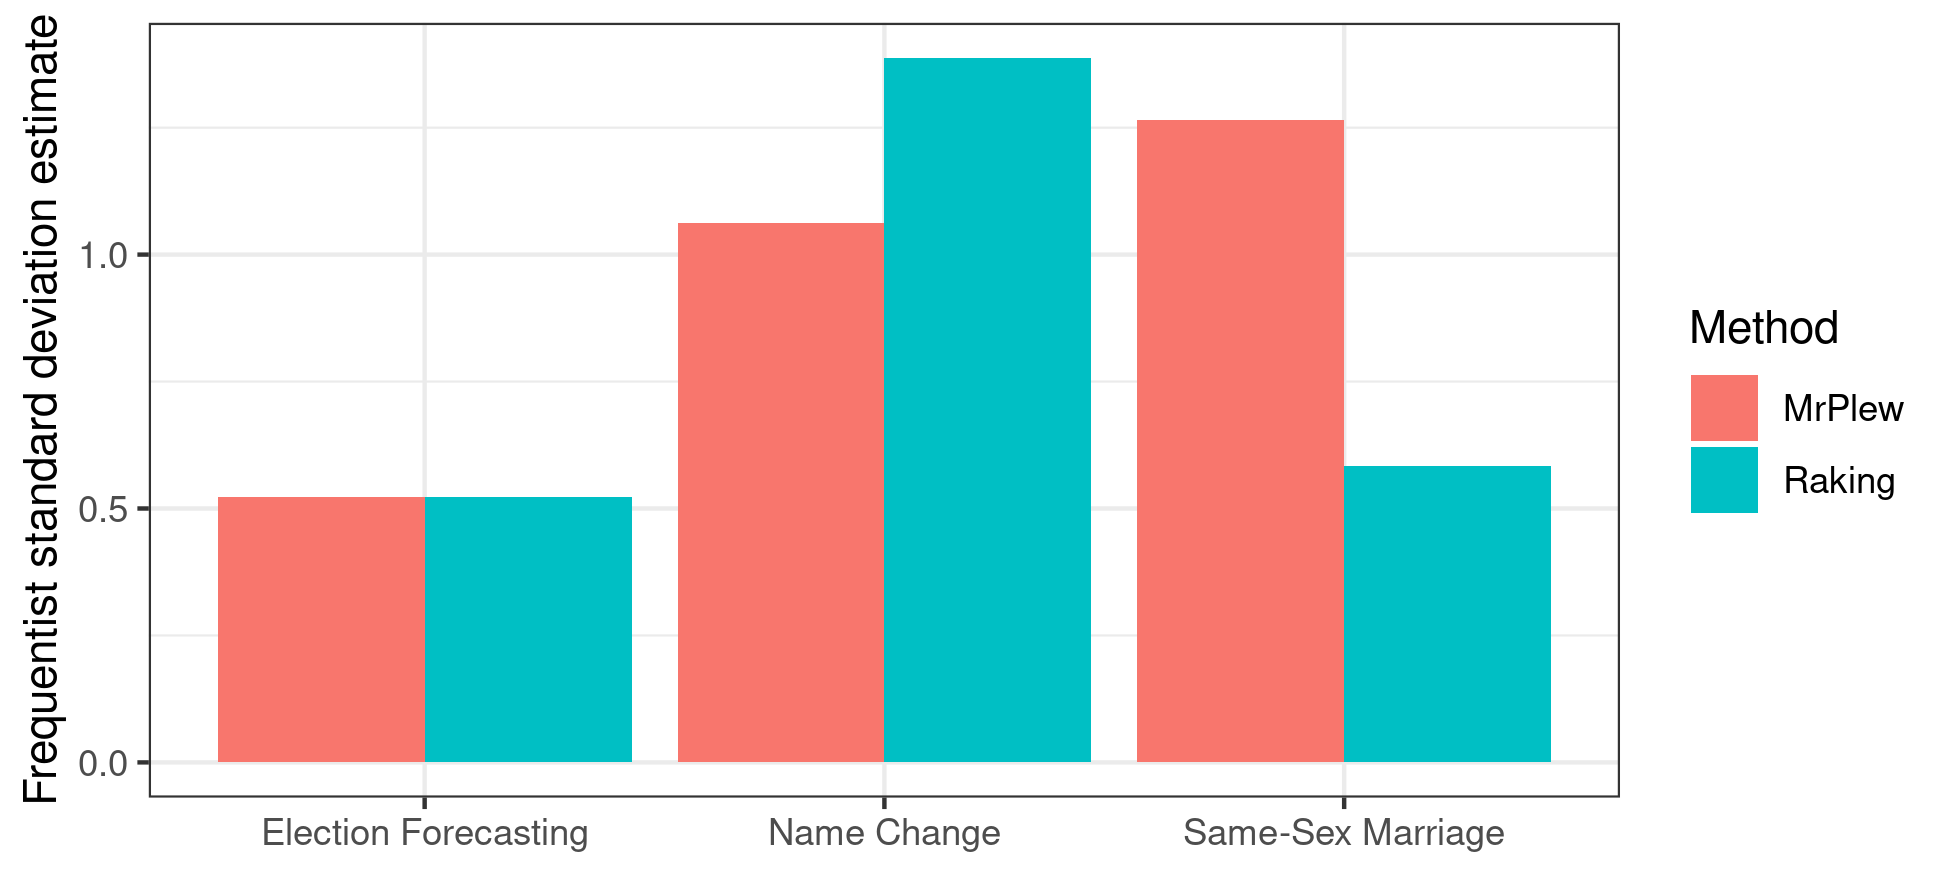
\includegraphics[width=0.98\linewidth,height=0.441\linewidth]{figure/varplot-1} 

}

\caption[]{Estimates of the frequentist standard deviation of $\sqrt{\nsur} \muhat[\mrp]$ and $\sqrt{\nsur} \muhat[\cal]$}\label{fig:varplot}
\end{figure}

\end{knitrout}
}


% fig.scap prevents math in the caption optional argument
\newcommand{\BootstrapPlot}{

\begin{knitrout}
\definecolor{shadecolor}{rgb}{0.969, 0.969, 0.969}\color{fgcolor}\begin{figure}[H]

{\centering 
\includegraphics[width=0.98\linewidth,height=0.441\linewidth]{figure/bootplot-1} 

}

\caption[]{Estimates of the frequentist standard deviation of $\sqrt{\nsur} \muhat[\mrp]$}\label{fig:bootplot}
\end{figure}

\end{knitrout}
}


% \newcommand{\WeightsPlot}{
% <<>>=
% figcap <- paste0("Comparison of weights")
% @
% <<weightsplot, cache=cache, fig.show='hold', fig.cap=figcap, fig.pos="H", fig.scap="">>=
% print(weight_plt)
% @
% }


\newcommand{\WeightsPlotLax}{

\begin{knitrout}
\definecolor{shadecolor}{rgb}{0.969, 0.969, 0.969}\color{fgcolor}\begin{figure}[H]

{\centering 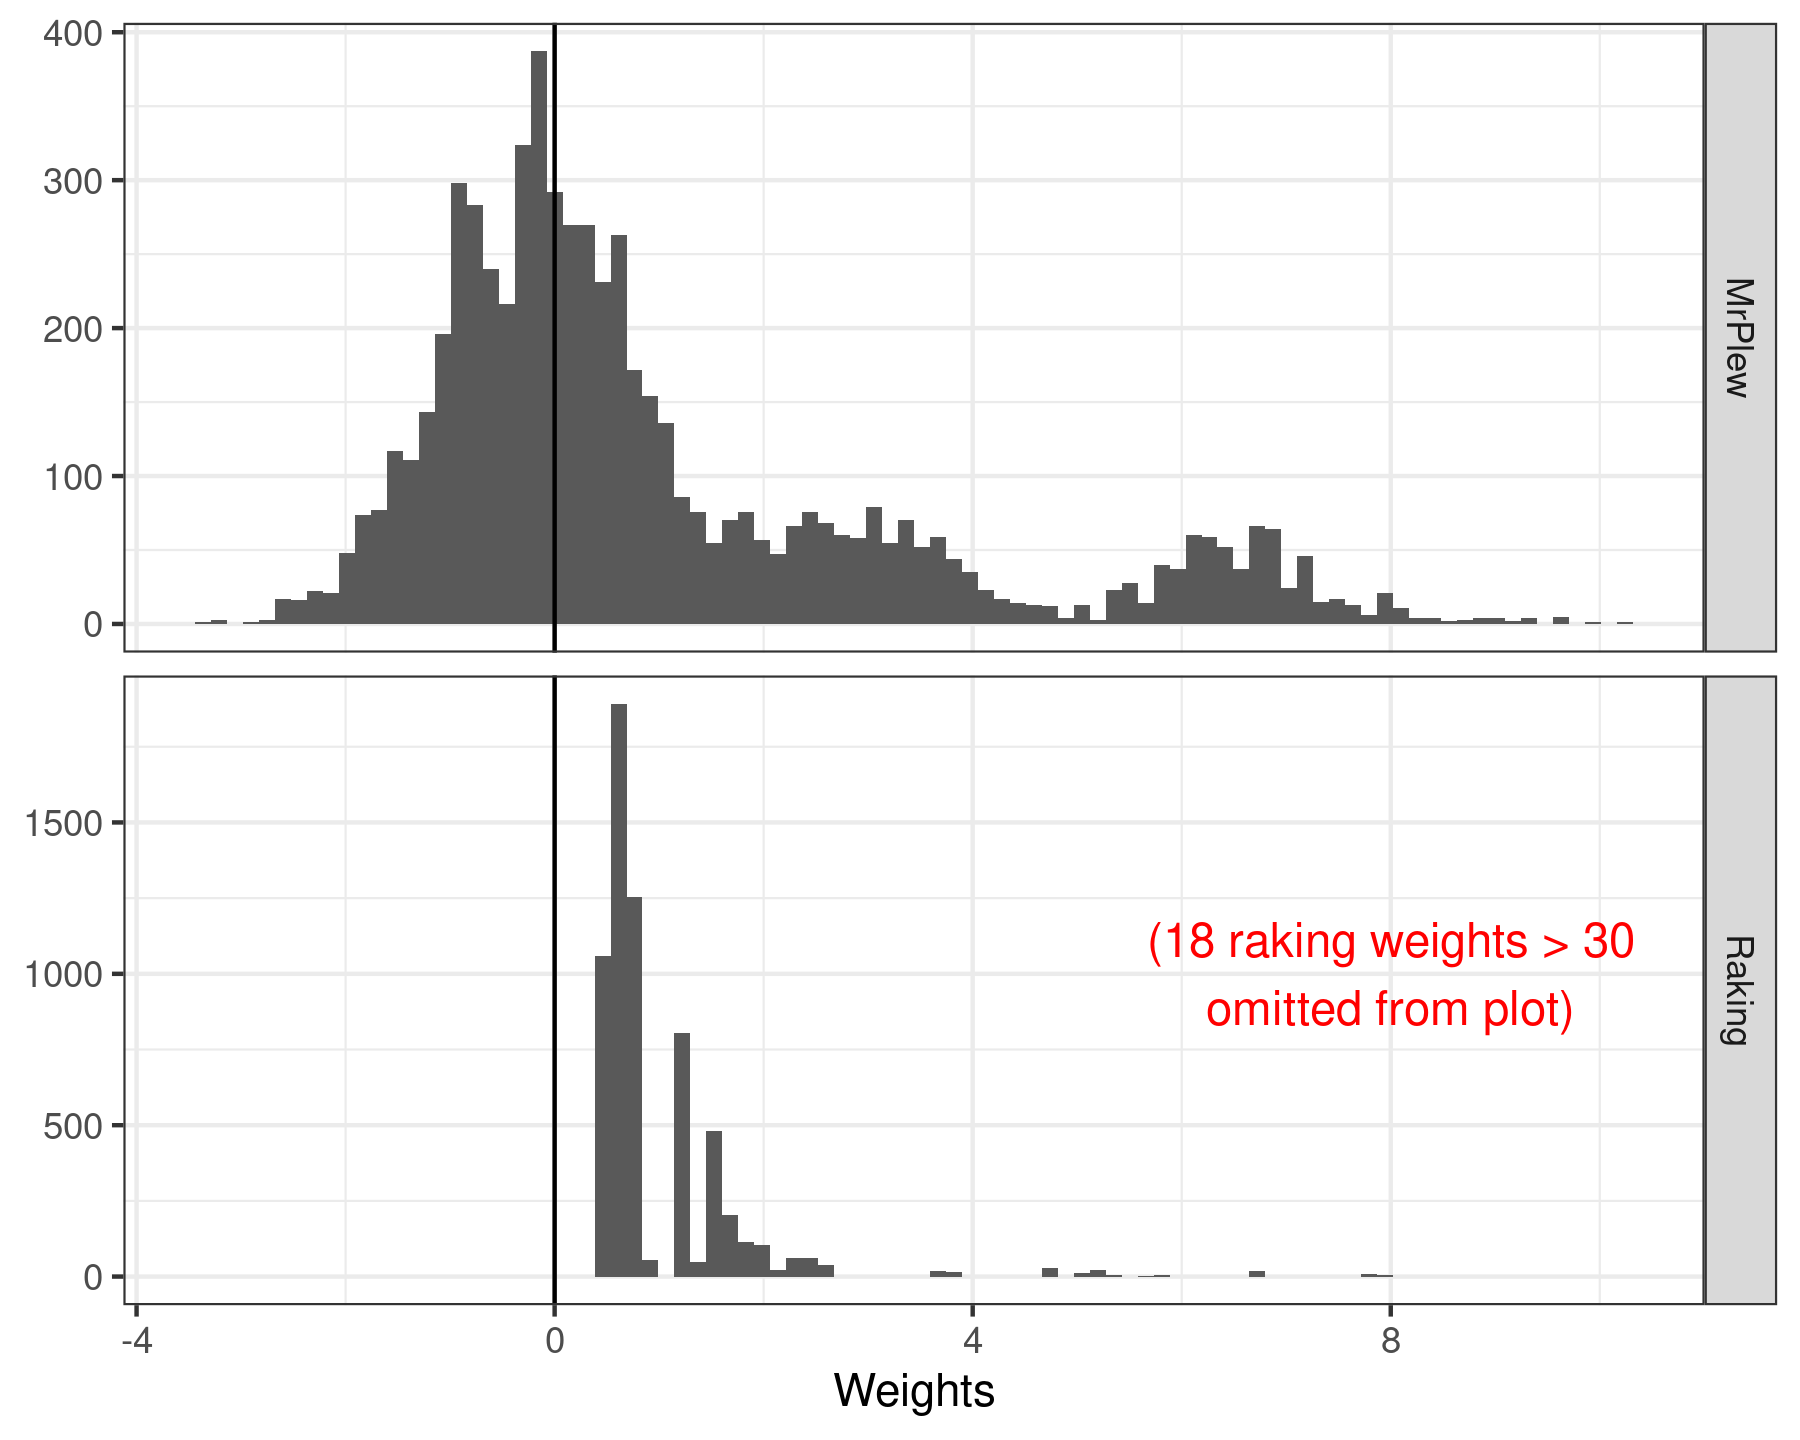
\includegraphics[width=0.98\linewidth,height=0.784\linewidth]{figure/weightsplotlax-1} 

}

\caption[]{Comparison of weights for the Same-Sex Marriage analysis}\label{fig:weightsplotlax}
\end{figure}

\end{knitrout}

}


\newcommand{\WeightsBivPlotLax}{

\begin{knitrout}
\definecolor{shadecolor}{rgb}{0.969, 0.969, 0.969}\color{fgcolor}\begin{figure}[H]

{\centering 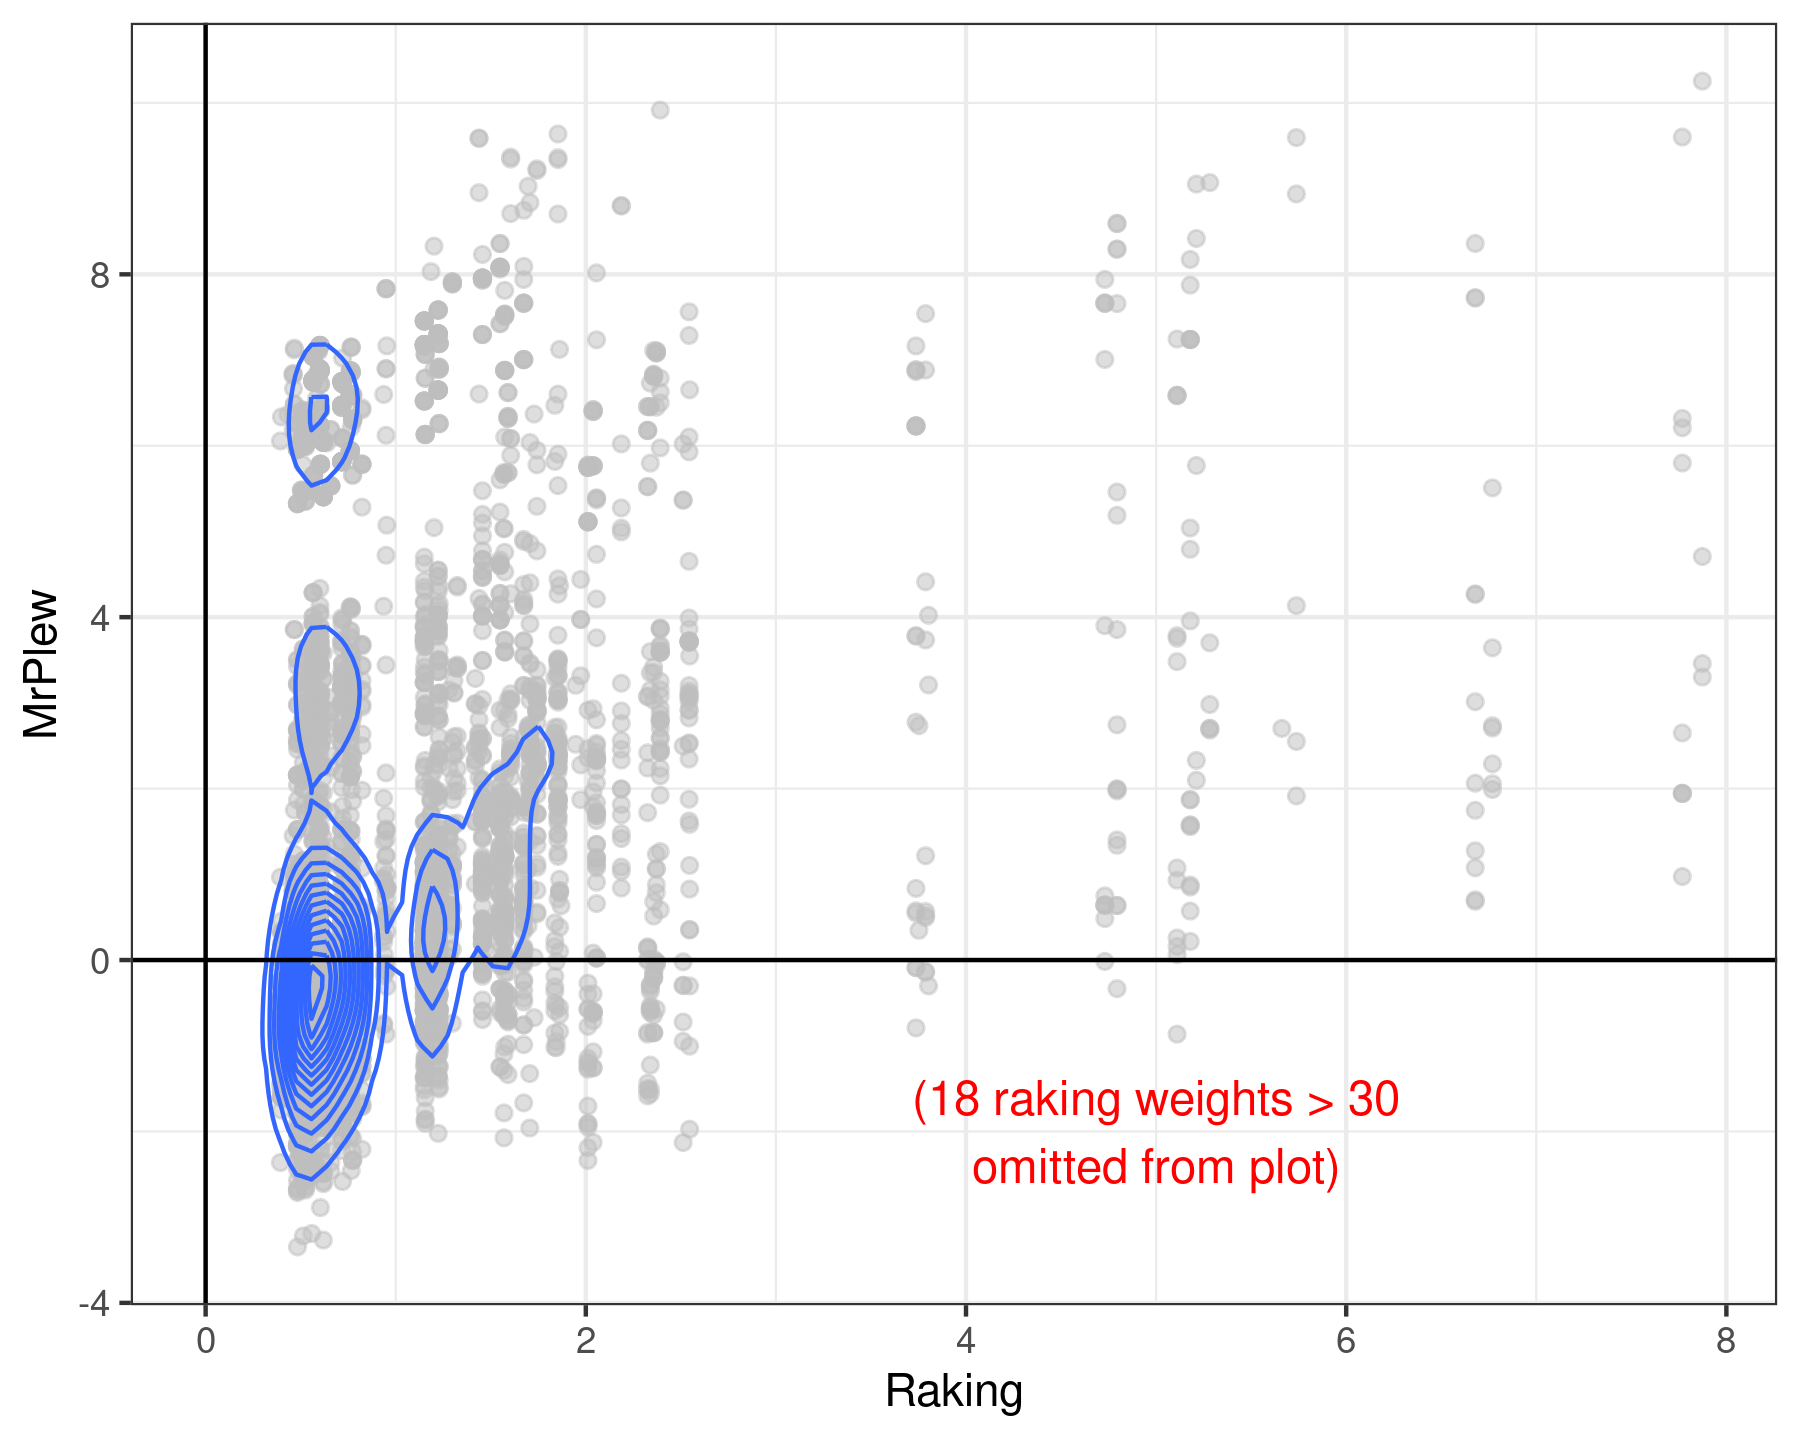
\includegraphics[width=0.98\linewidth,height=0.784\linewidth]{figure/weightsbivplotlax-1} 

}

\caption[]{Comparison of weights for the Same-Sex Marriage analysis}\label{fig:weightsbivplotlax}
\end{figure}

\end{knitrout}

}


\newcommand{\VarPlotLax}{

\begin{knitrout}
\definecolor{shadecolor}{rgb}{0.969, 0.969, 0.969}\color{fgcolor}

{\centering 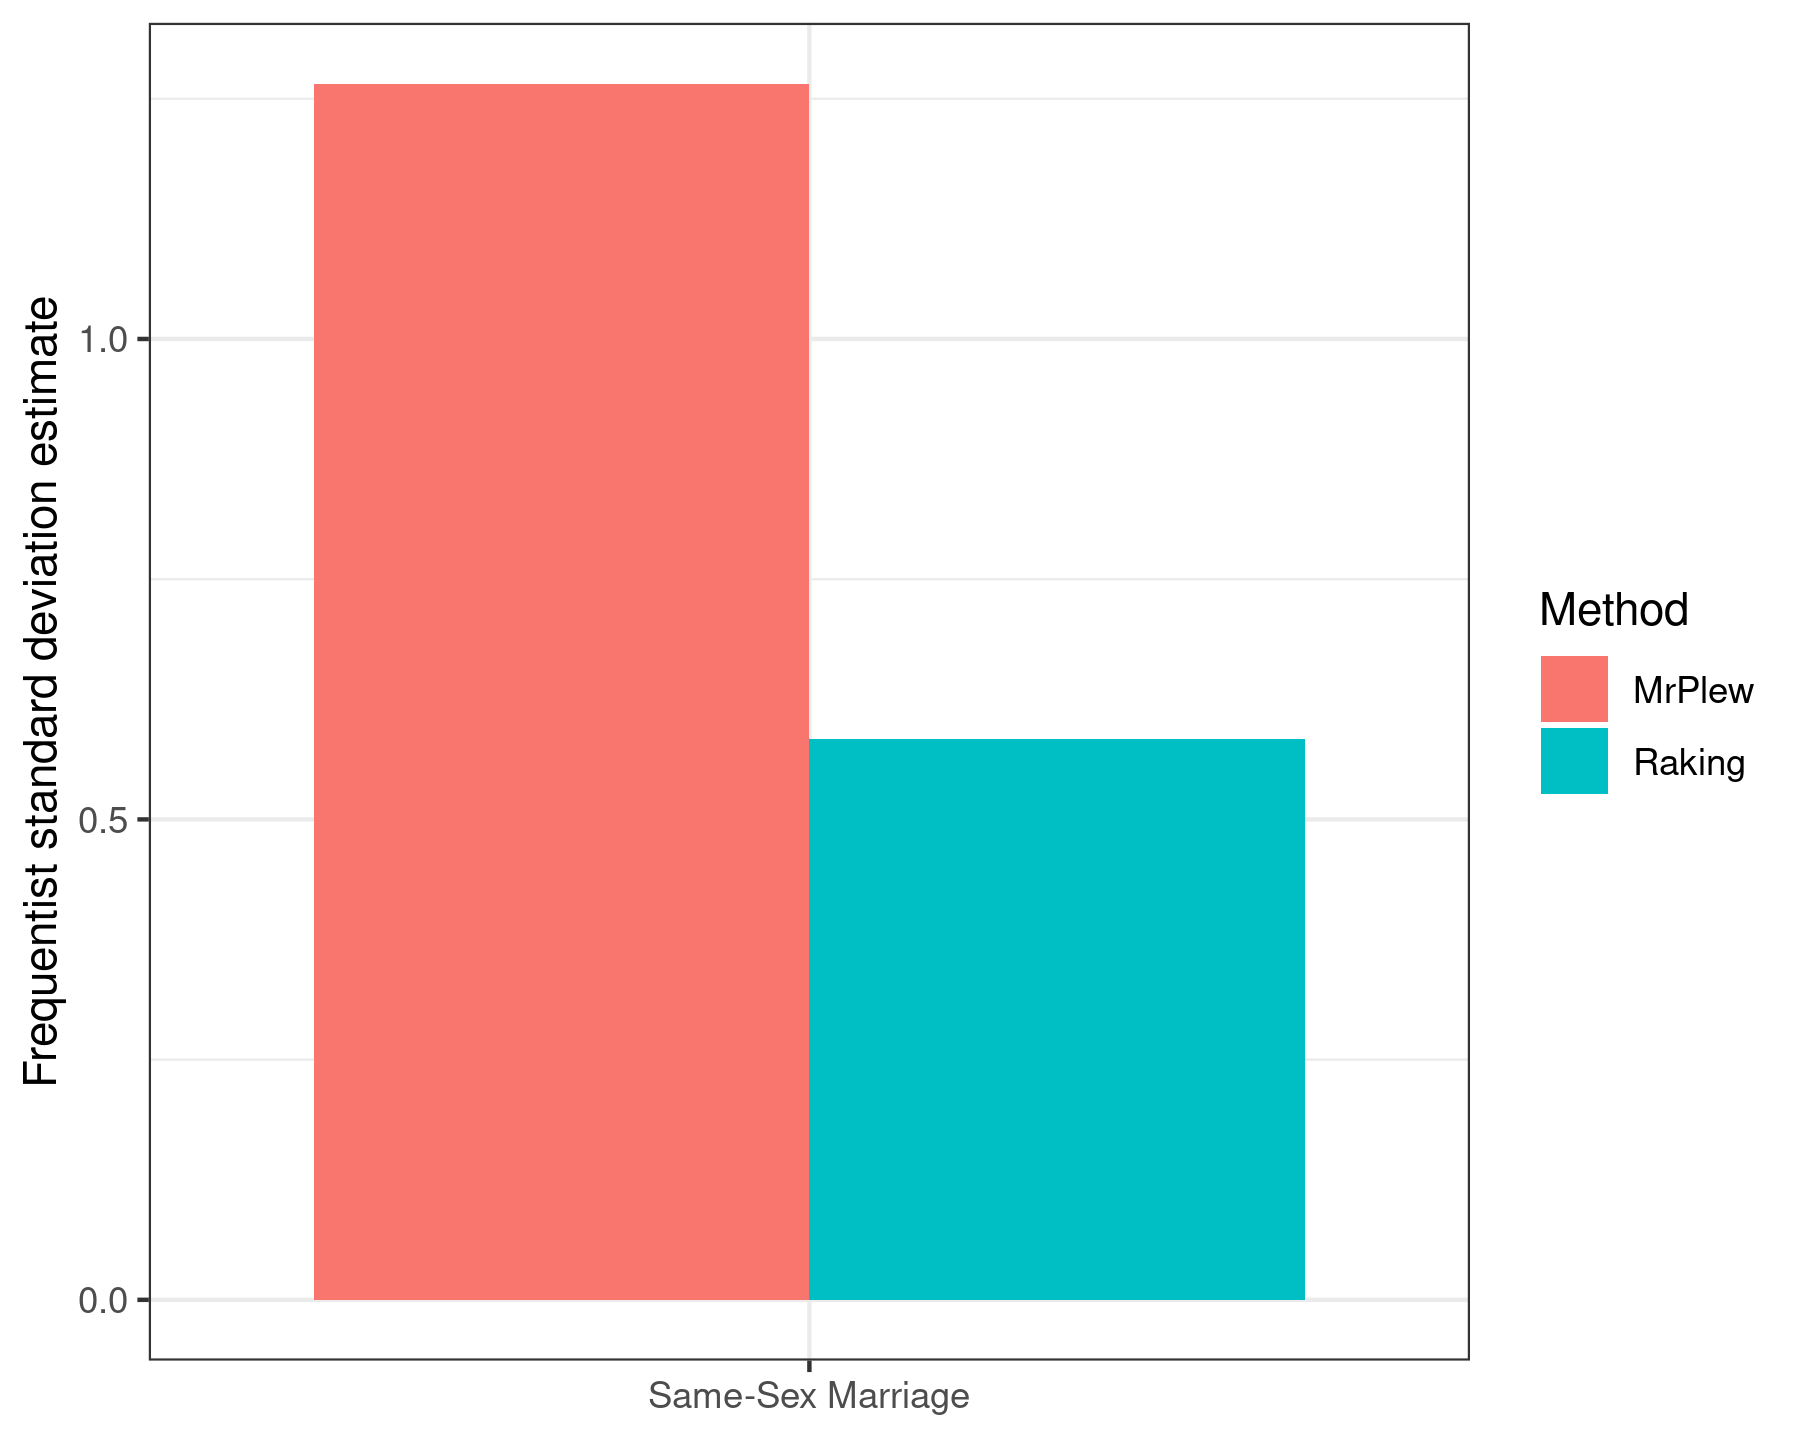
\includegraphics[width=0.98\linewidth,height=0.784\linewidth]{figure/varplotlax-1} 

}


\end{knitrout}

}


\newcommand{\BayesVarPlotLax}{

\begin{knitrout}
\definecolor{shadecolor}{rgb}{0.969, 0.969, 0.969}\color{fgcolor}

{\centering 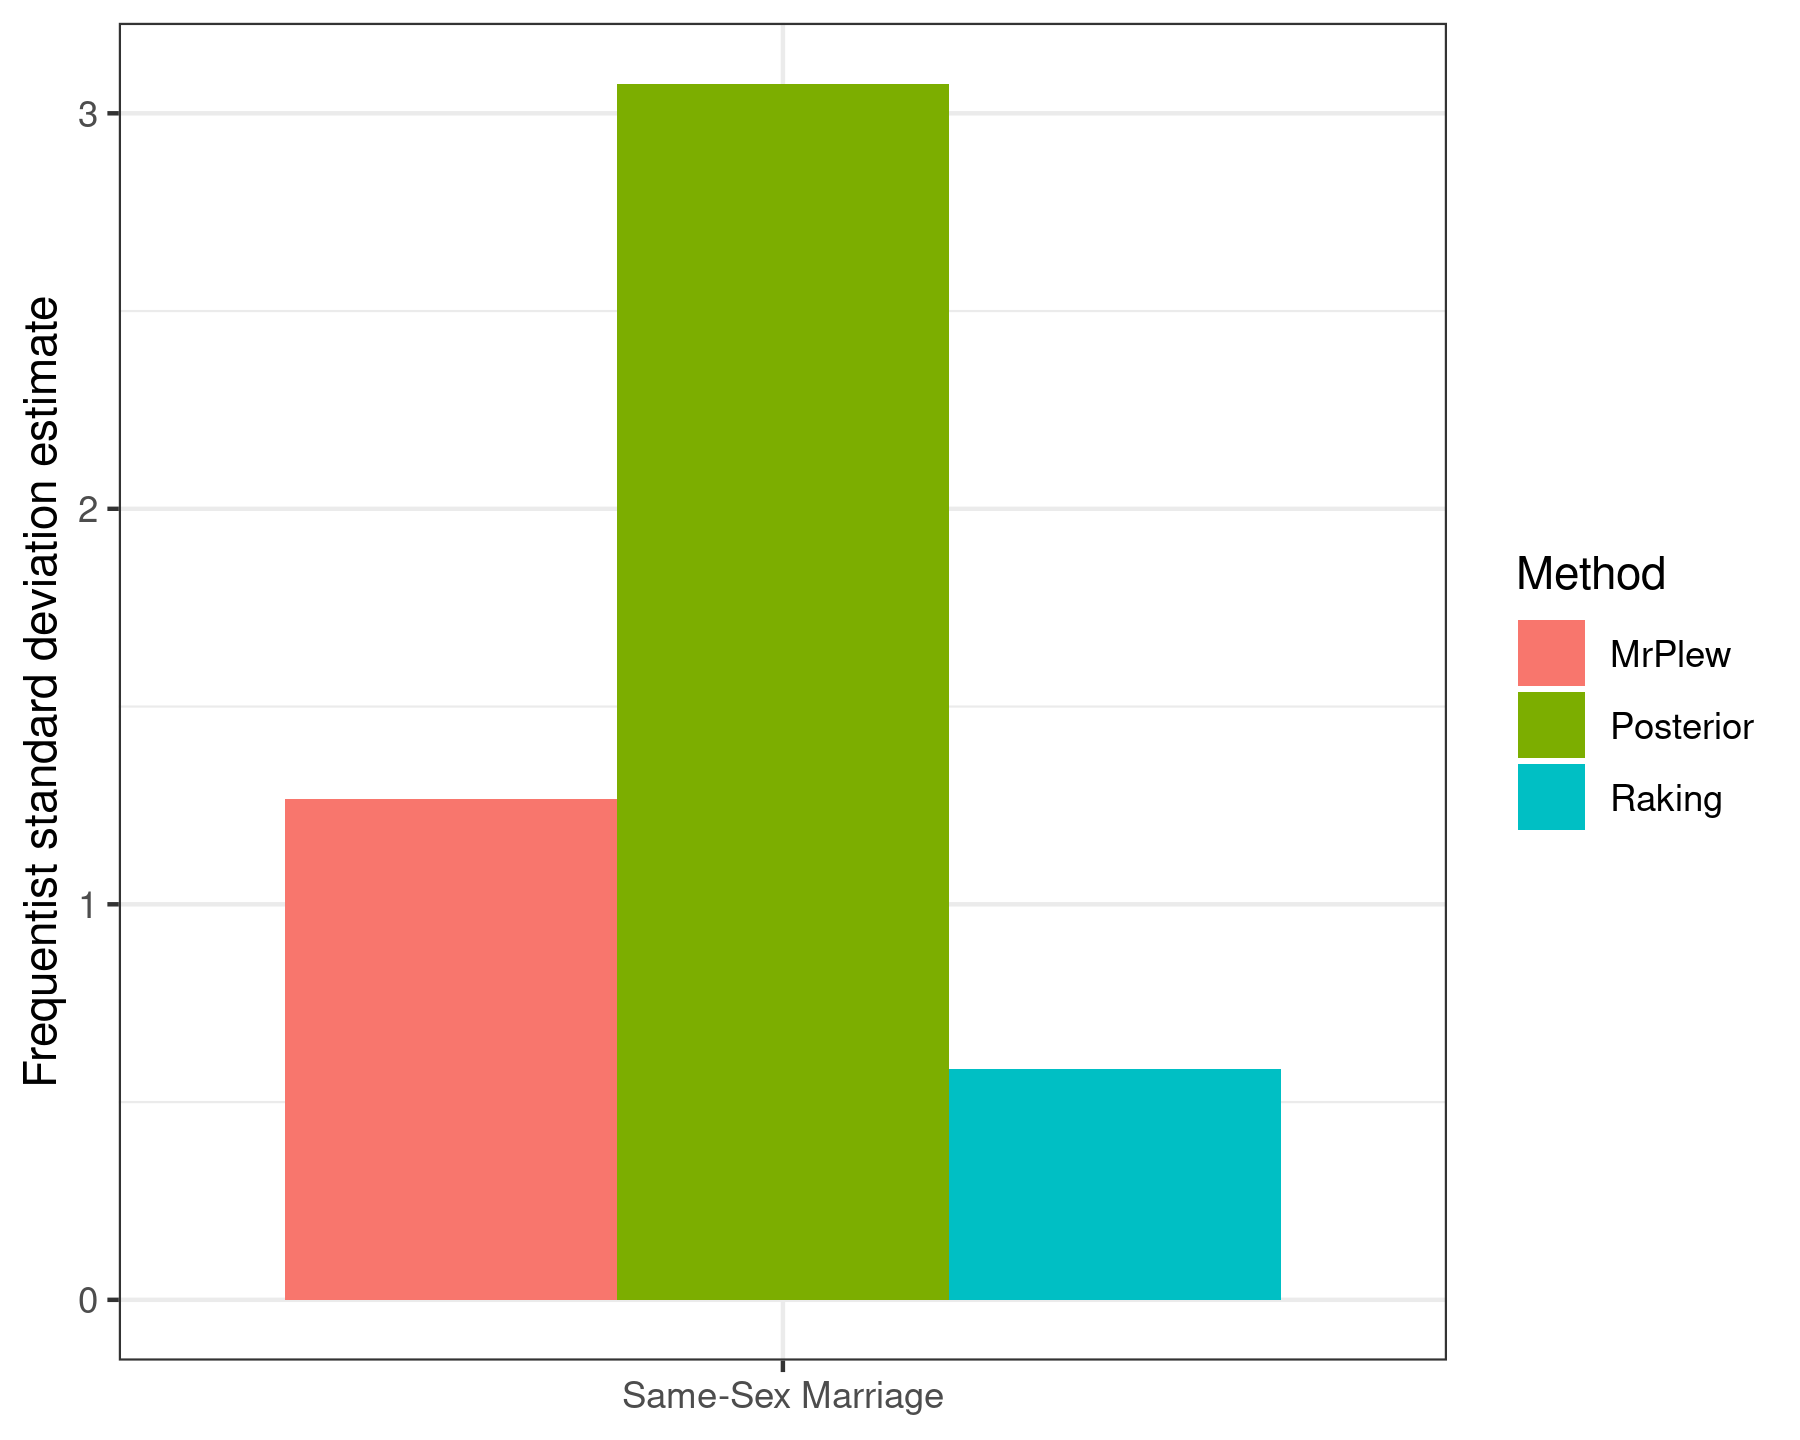
\includegraphics[width=0.98\linewidth,height=0.784\linewidth]{figure/bayesvarplotlax-1} 

}


\end{knitrout}

}



%%%%%%%%%%%%%%%%%%%%%%%%%%%%%%%%%%%%%%%%5
% Balance plots

% \newcommand{\AlexanderBalance}{
% <<>>=
% figcap <- paste0("Balance")
% @
% <<alexanderbalanceplot, cache=cache, fig.show='hold', fig.cap=figcap, fig.pos="H", fig.scap="">>=
% PlotBalanceForEnv(alexander, interactions=FALSE)
% @
% }


% \newcommand{\AlexanderBalanceInteractions}{
% <<>>=
% figcap <- paste0("Balance")
% @
% <<alexanderbalanceplotinteractions, cache=cache, fig.show='hold', fig.cap=figcap, fig.pos="H", fig.scap="">>=
% PlotBalanceForEnv(alexander, interactions=TRUE, threshold=3)
% @
% }



\newcommand{\LaxphilipsBalance}{

\begin{knitrout}
\definecolor{shadecolor}{rgb}{0.969, 0.969, 0.969}\color{fgcolor}

{\centering 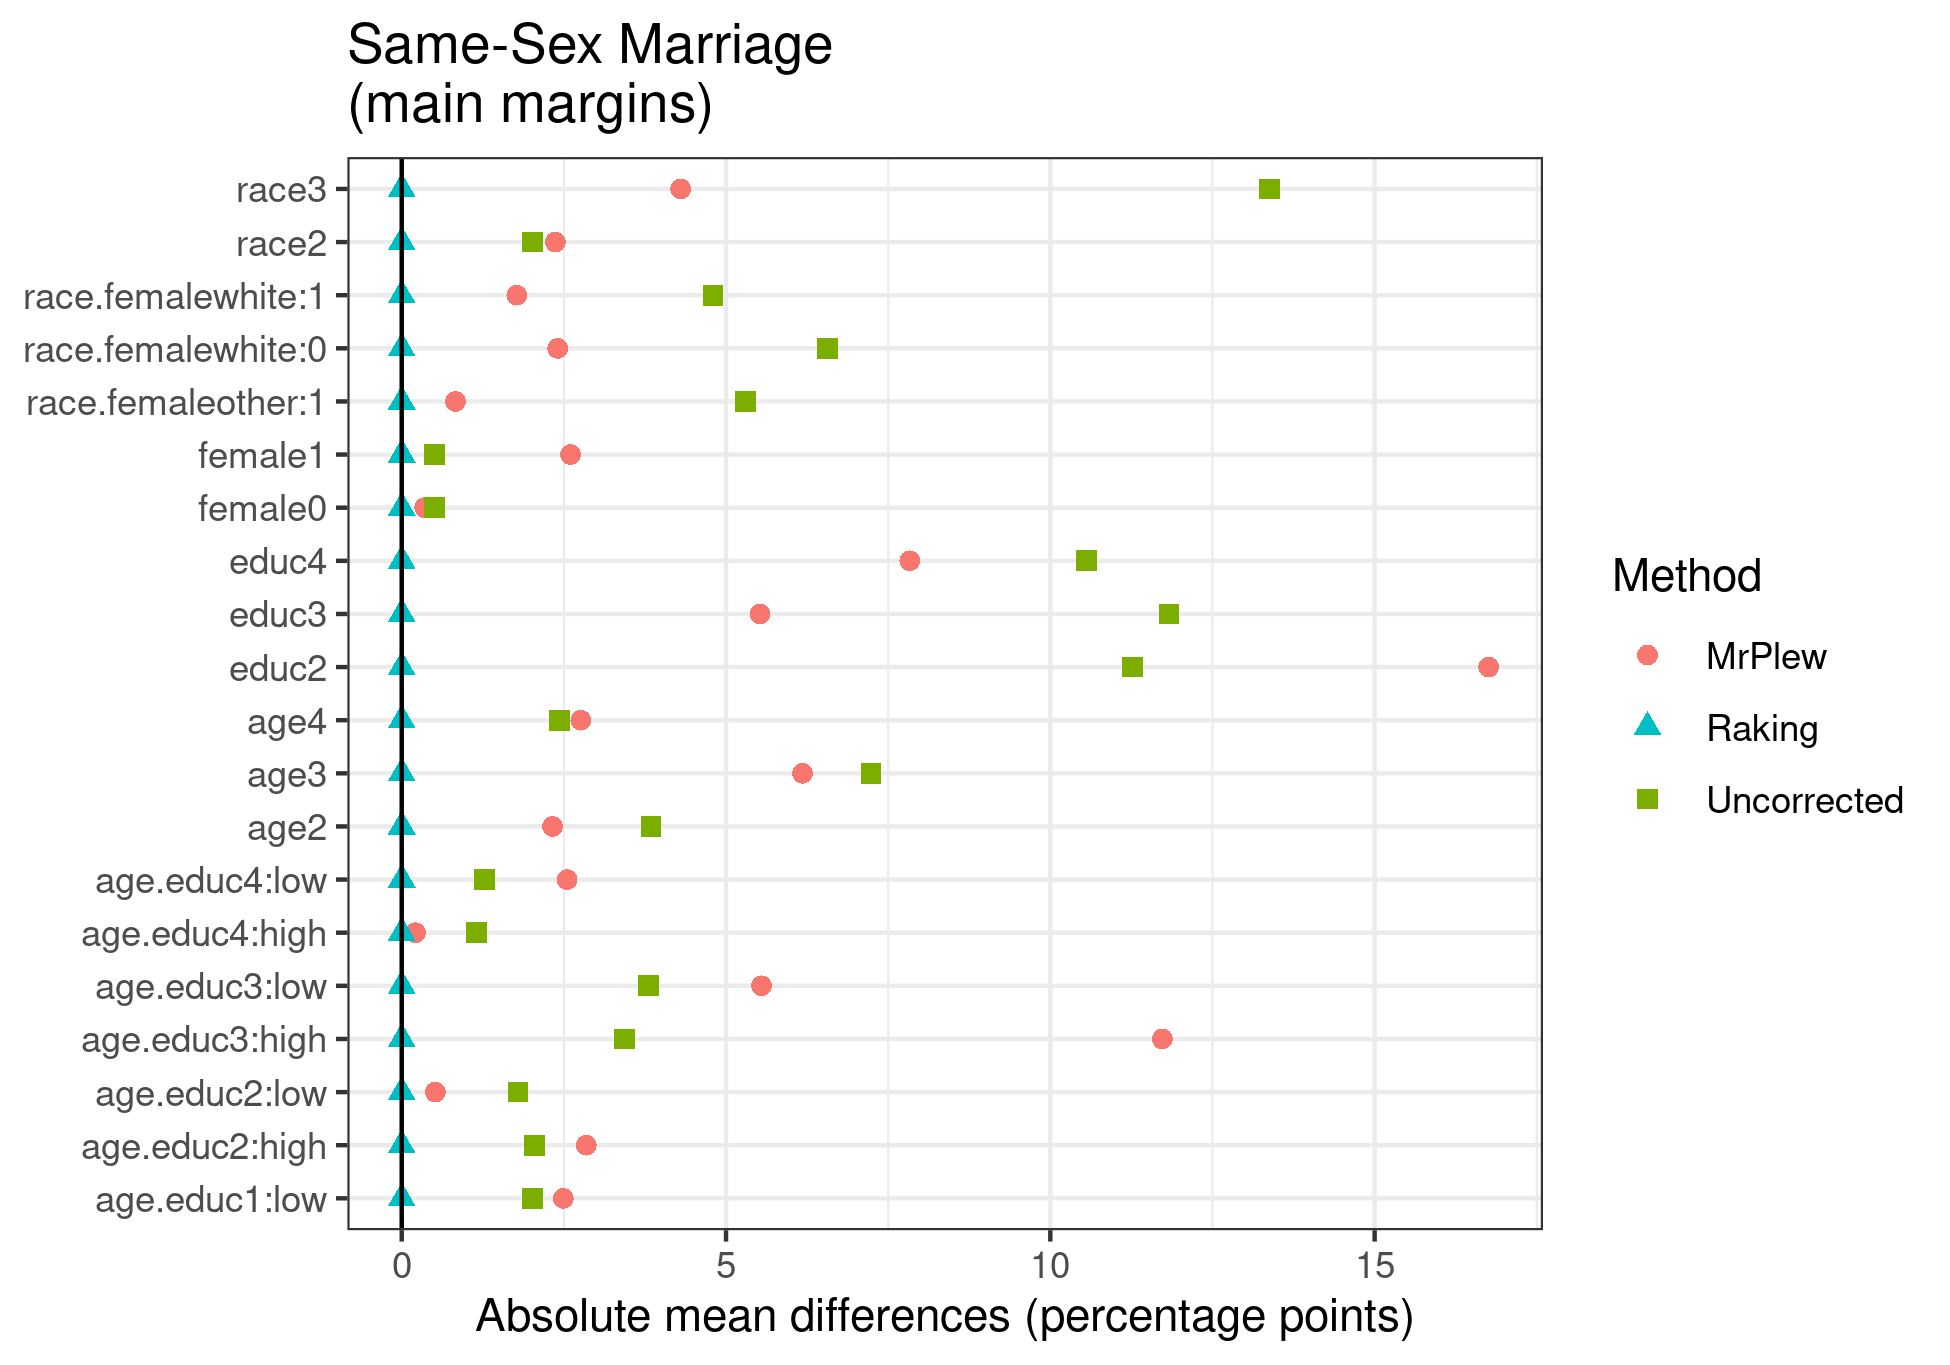
\includegraphics[width=0.98\linewidth,height=0.686\linewidth]{figure/laxphilipsbalanceplot-1} 

}


\end{knitrout}

}

\newcommand{\LaxphilipsBalanceInteractions}{

\begin{knitrout}
\definecolor{shadecolor}{rgb}{0.969, 0.969, 0.969}\color{fgcolor}

{\centering 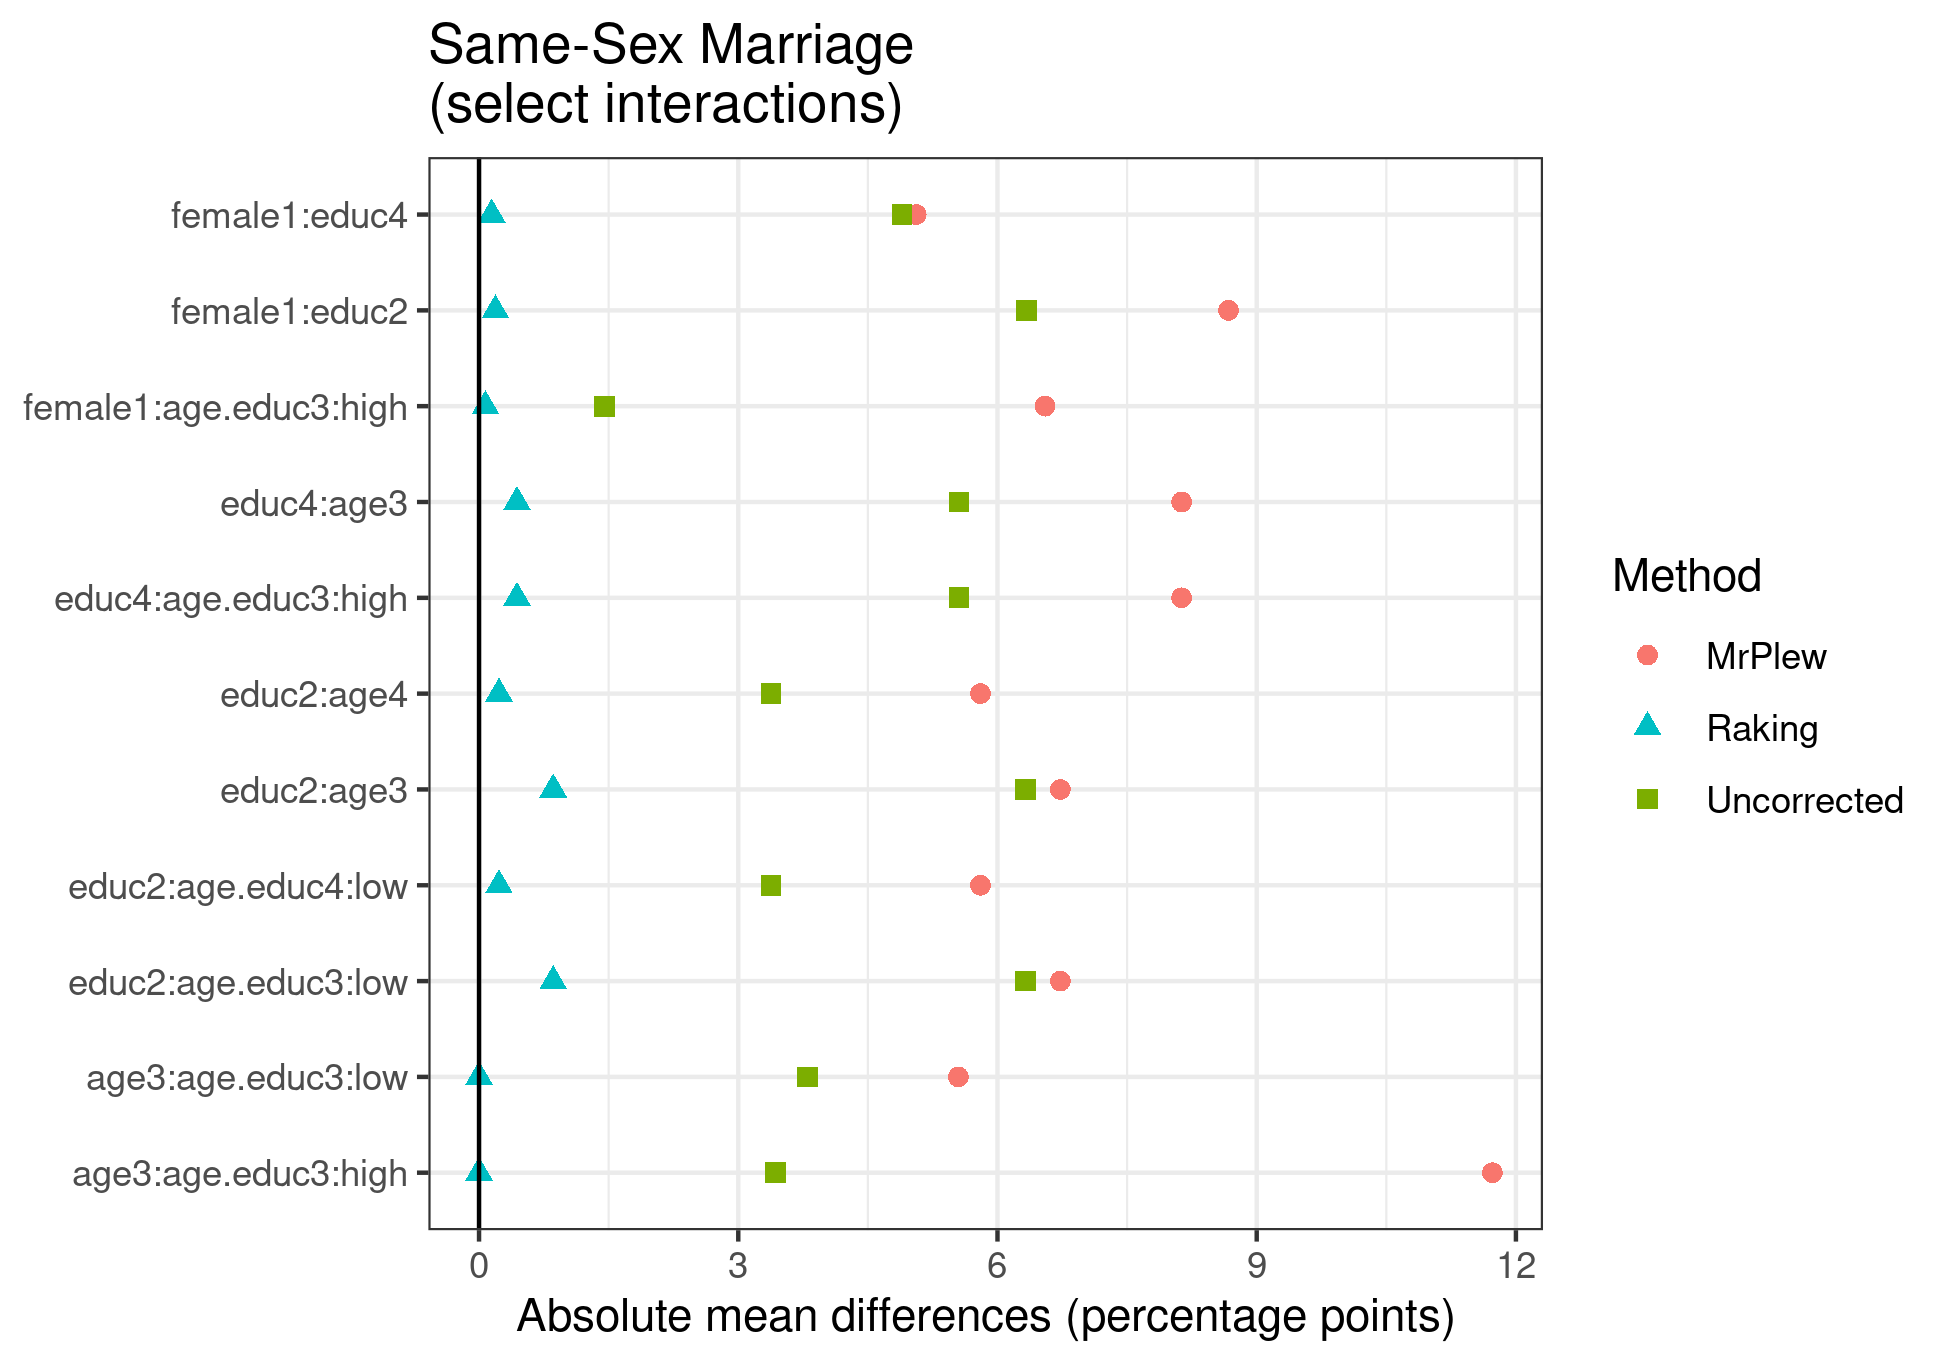
\includegraphics[width=0.98\linewidth,height=0.686\linewidth]{figure/laxphilipsbalanceplotinteractions-1} 

}


\end{knitrout}

}


% \newcommand{\StoriesBalance}{
% <<>>=
% figcap <- paste0("Balance")
% @
% <<storiesbalanceplot, cache=cache, fig.show='hold', fig.cap=figcap, fig.pos="H", fig.scap="">>=
% PlotBalanceForEnv(stories, interactions=FALSE)
% @
% }



% \newcommand{\StoriesBalanceInteractions}{
% <<>>=
% figcap <- paste0("Balance")
% @
% <<storiesbalanceplotinteractions, cache=cache, fig.show='hold', fig.cap=figcap, fig.pos="H", fig.scap="">>=
% PlotBalanceForEnv(stories, interactions=TRUE, threshold=0.5)
% @
% }




%%%%%%%%%%%%%%%%%%%%%%%%%%%%%%%%%%%%%%%%%%%%%%%%





\newcommand{\AlexanderRefitPlot}{

\begin{knitrout}
\definecolor{shadecolor}{rgb}{0.969, 0.969, 0.969}\color{fgcolor}\begin{figure}[H]

{\centering 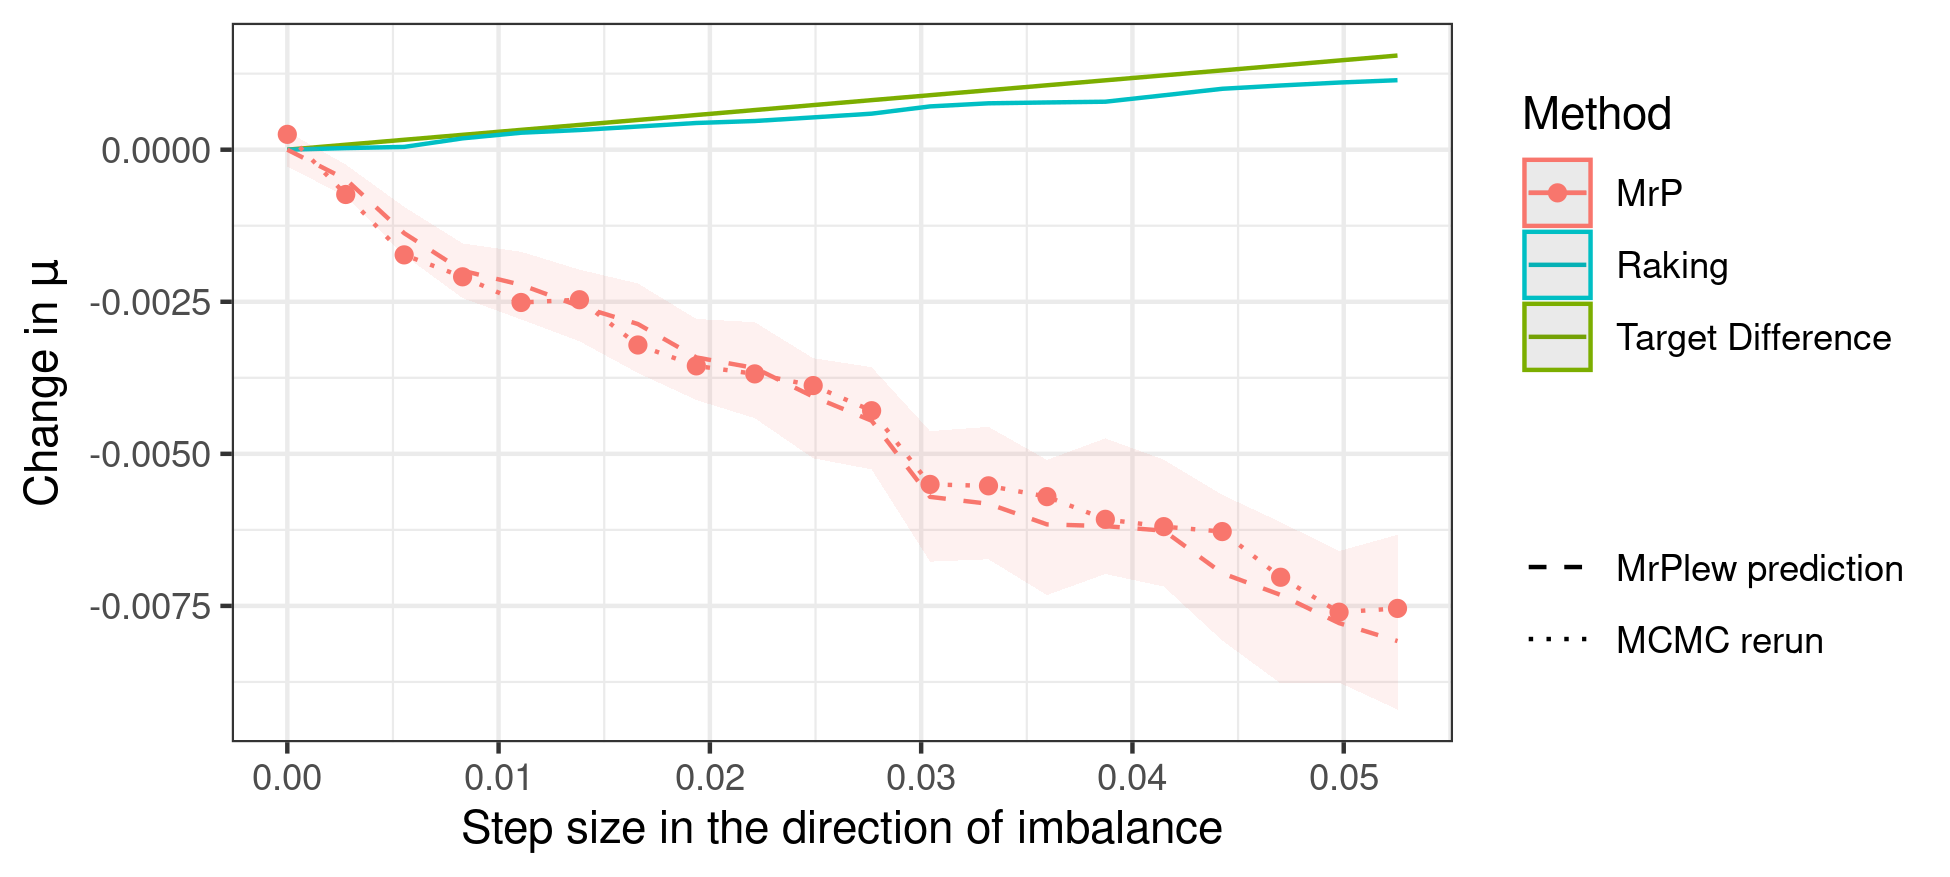
\includegraphics[width=0.98\linewidth,height=0.441\linewidth]{figure/alexanderrefitplot-1} 

}

\caption[]{Refit}\label{fig:alexanderrefitplot}
\end{figure}

\end{knitrout}
}


\newcommand{\LaxRefitPlot}{

\begin{knitrout}
\definecolor{shadecolor}{rgb}{0.969, 0.969, 0.969}\color{fgcolor}\begin{figure}[H]

{\centering 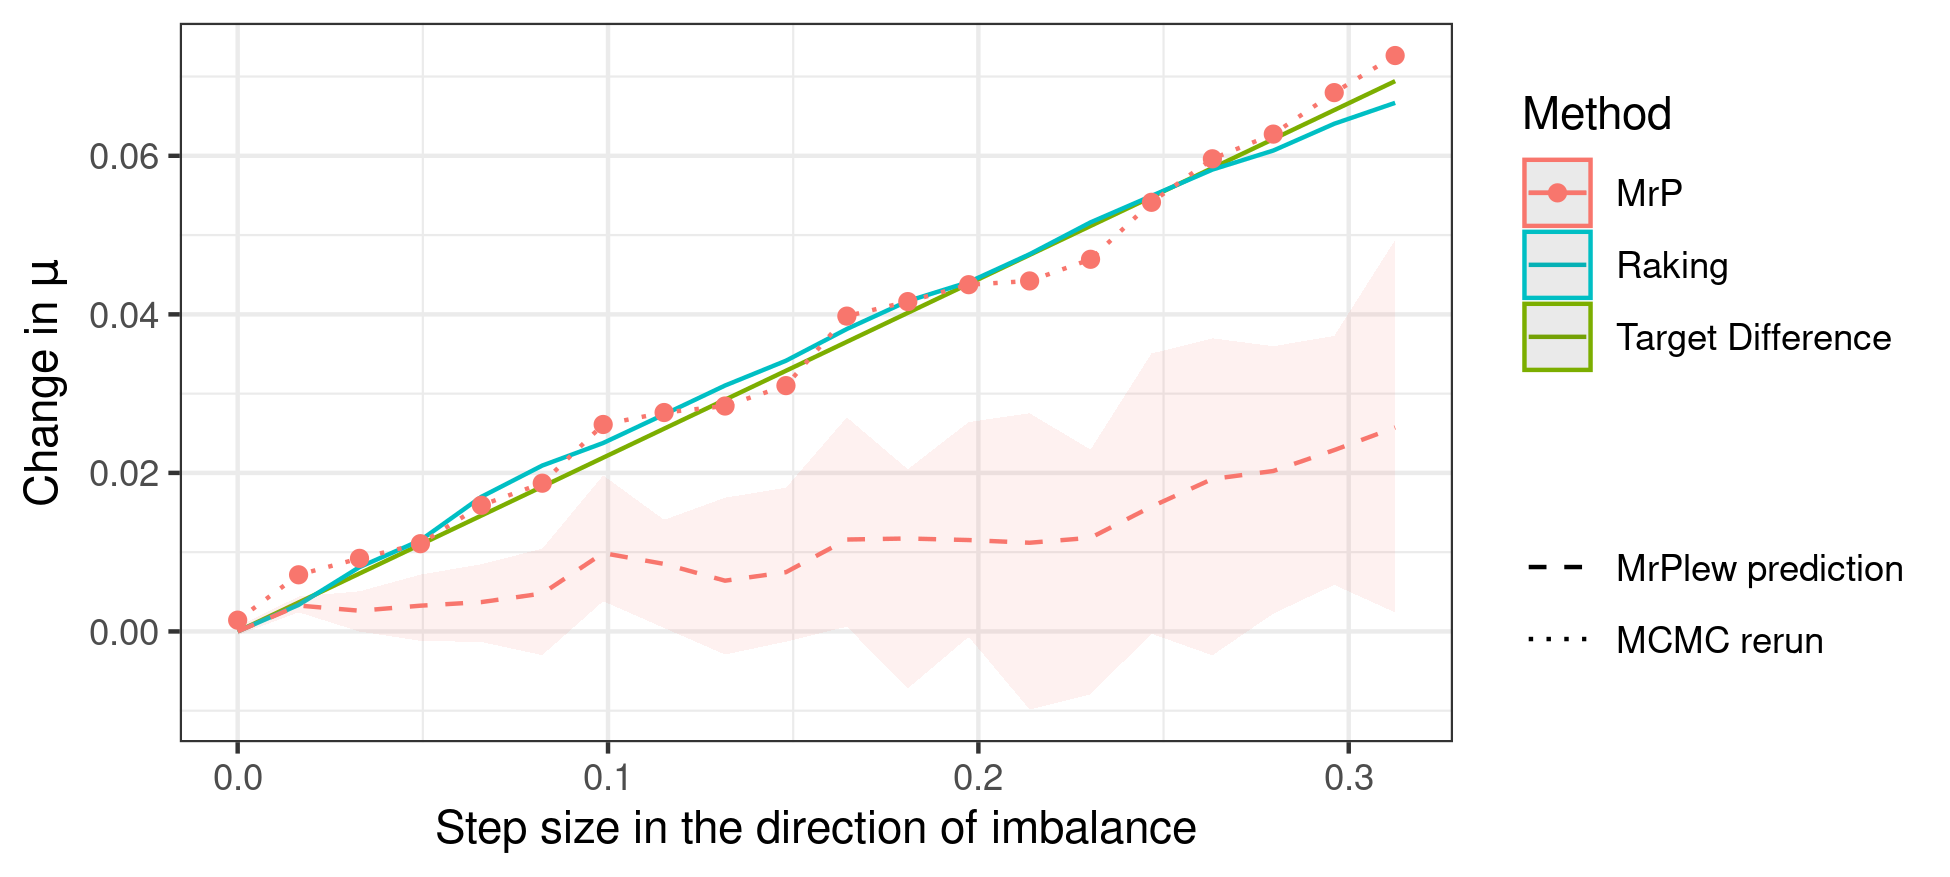
\includegraphics[width=0.98\linewidth,height=0.441\linewidth]{figure/laxphilipsrefitplot-1} 

}

\caption[]{Refit}\label{fig:laxphilipsrefitplot}
\end{figure}

\end{knitrout}
}




\newcommand{\LaxphilipsCAPoolingPlot}{

\begin{knitrout}
\definecolor{shadecolor}{rgb}{0.969, 0.969, 0.969}\color{fgcolor}\begin{figure}[H]

{\centering 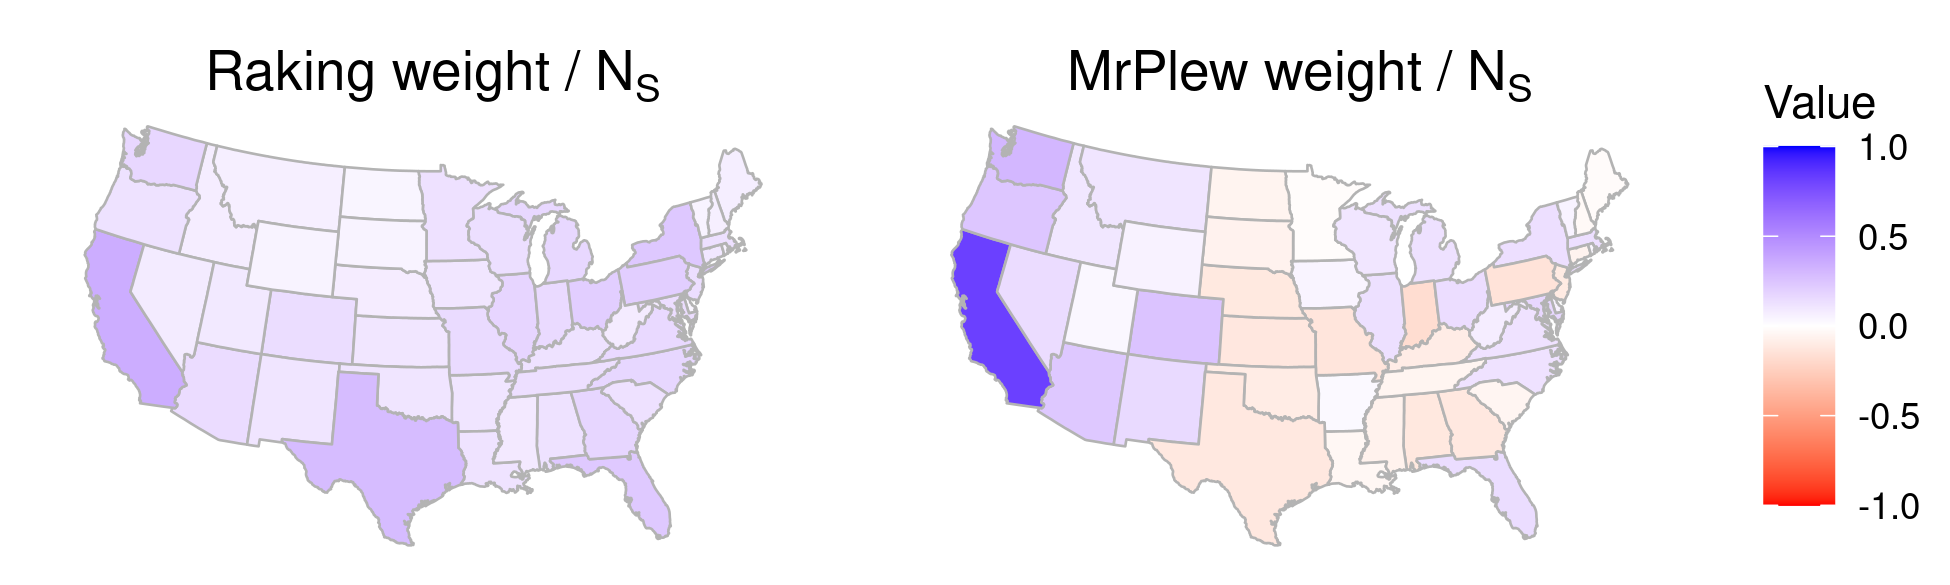
\includegraphics[width=0.98\linewidth,height=0.294\linewidth]{figure/laxphilipscapoolingplot-1} 

}

\caption[]{Subgroup contribution for Same-Sex Marriage in California}\label{fig:laxphilipscapoolingplot}
\end{figure}

\end{knitrout}

}


\newcommand{\LaxphilipsMOPoolingPlot}{

\begin{knitrout}
\definecolor{shadecolor}{rgb}{0.969, 0.969, 0.969}\color{fgcolor}\begin{figure}[H]

{\centering 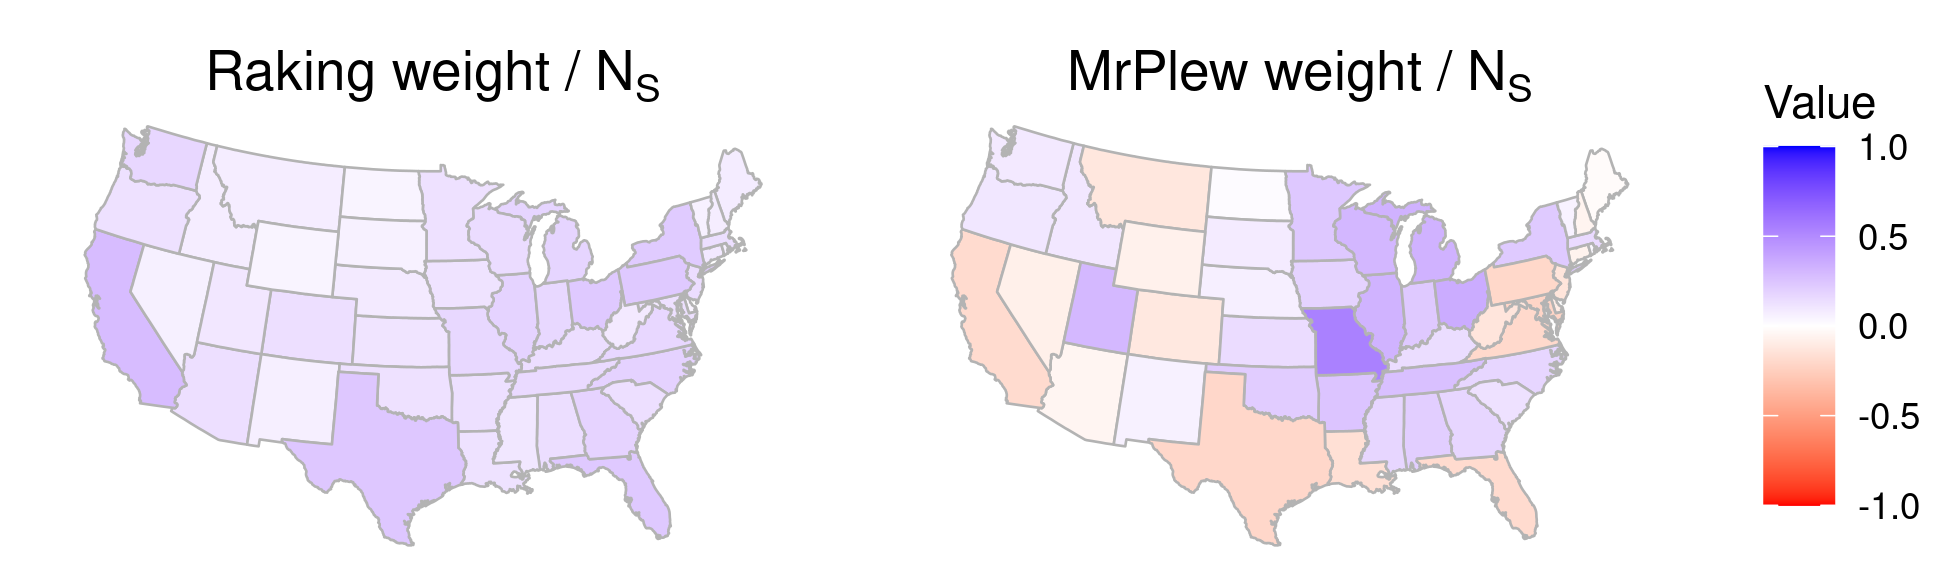
\includegraphics[width=0.98\linewidth,height=0.294\linewidth]{figure/laxphilipsmopoolingplot-1} 

}

\caption[]{Subgroup contribution for Same-Sex Marriage in Missouri}\label{fig:laxphilipsmopoolingplot}
\end{figure}

\end{knitrout}

}




\newcommand{\AlexanderPoolingPlot}{

\begin{knitrout}
\definecolor{shadecolor}{rgb}{0.969, 0.969, 0.969}\color{fgcolor}\begin{figure}[H]

{\centering 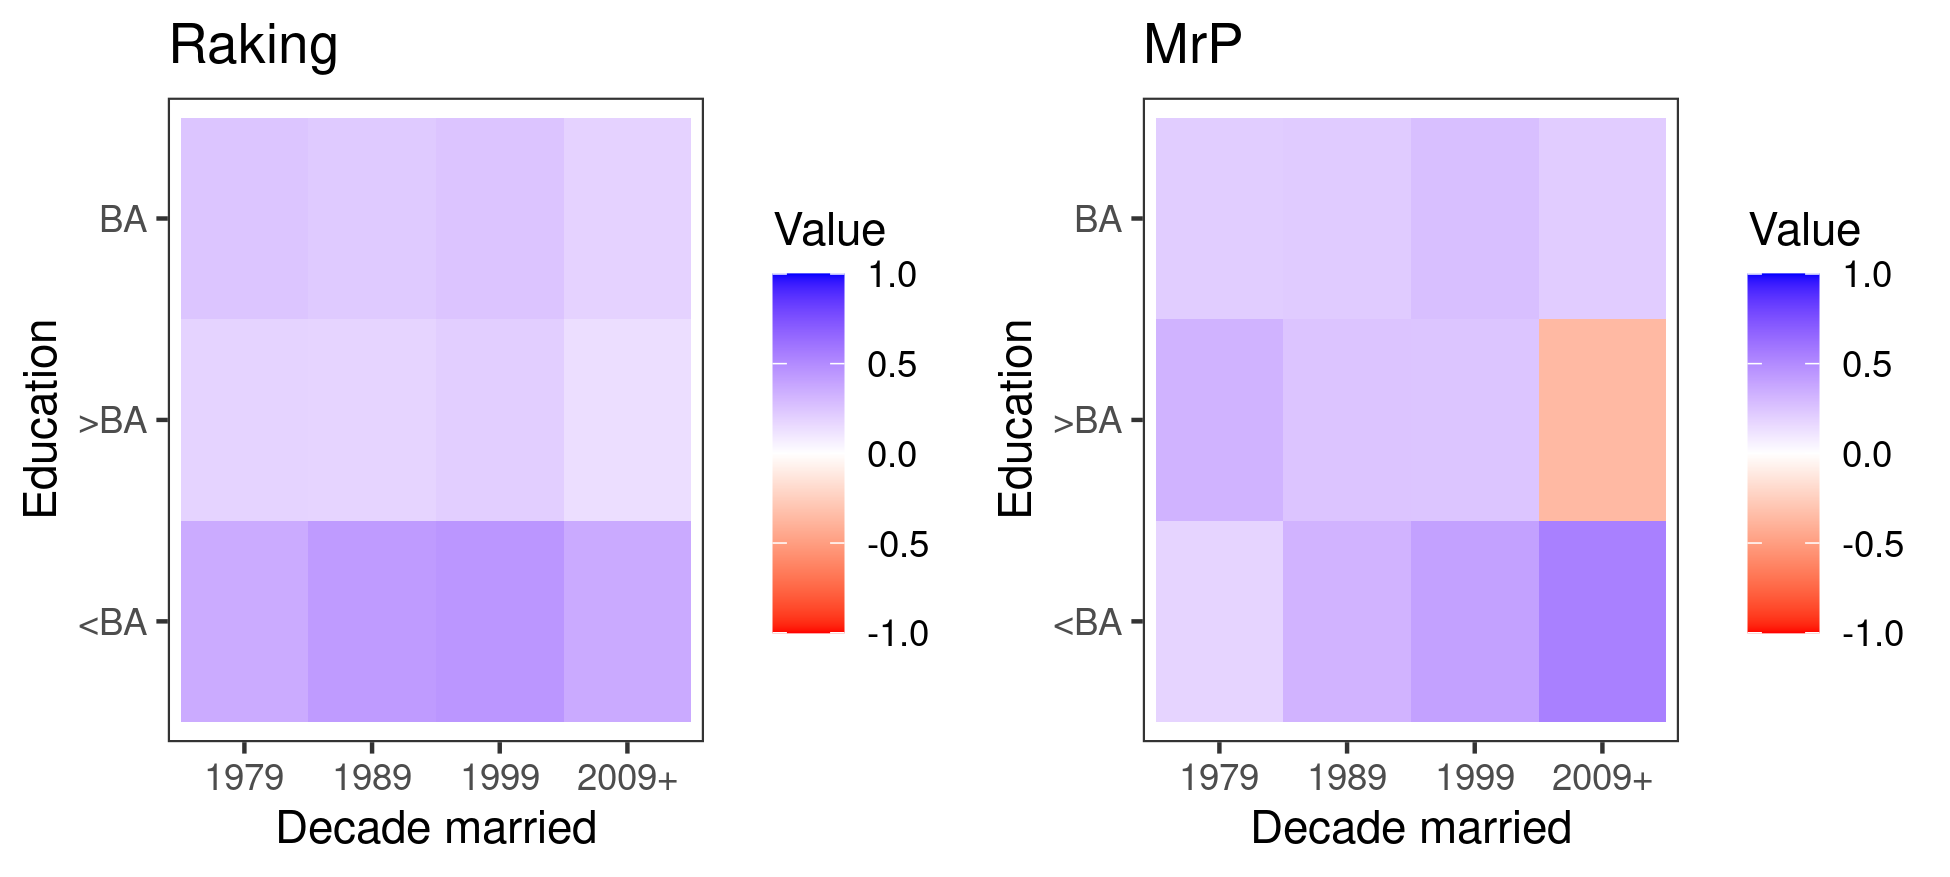
\includegraphics[width=0.98\linewidth,height=0.441\linewidth]{figure/alexanderpoolingplot-1} 

}

\caption[]{Subgroup contribution for Name Change}\label{fig:alexanderpoolingplot}
\end{figure}

\end{knitrout}
}


\newcommand{\PoolingComparisonPlot}{

\begin{knitrout}
\definecolor{shadecolor}{rgb}{0.969, 0.969, 0.969}\color{fgcolor}\begin{figure}[H]

{\centering 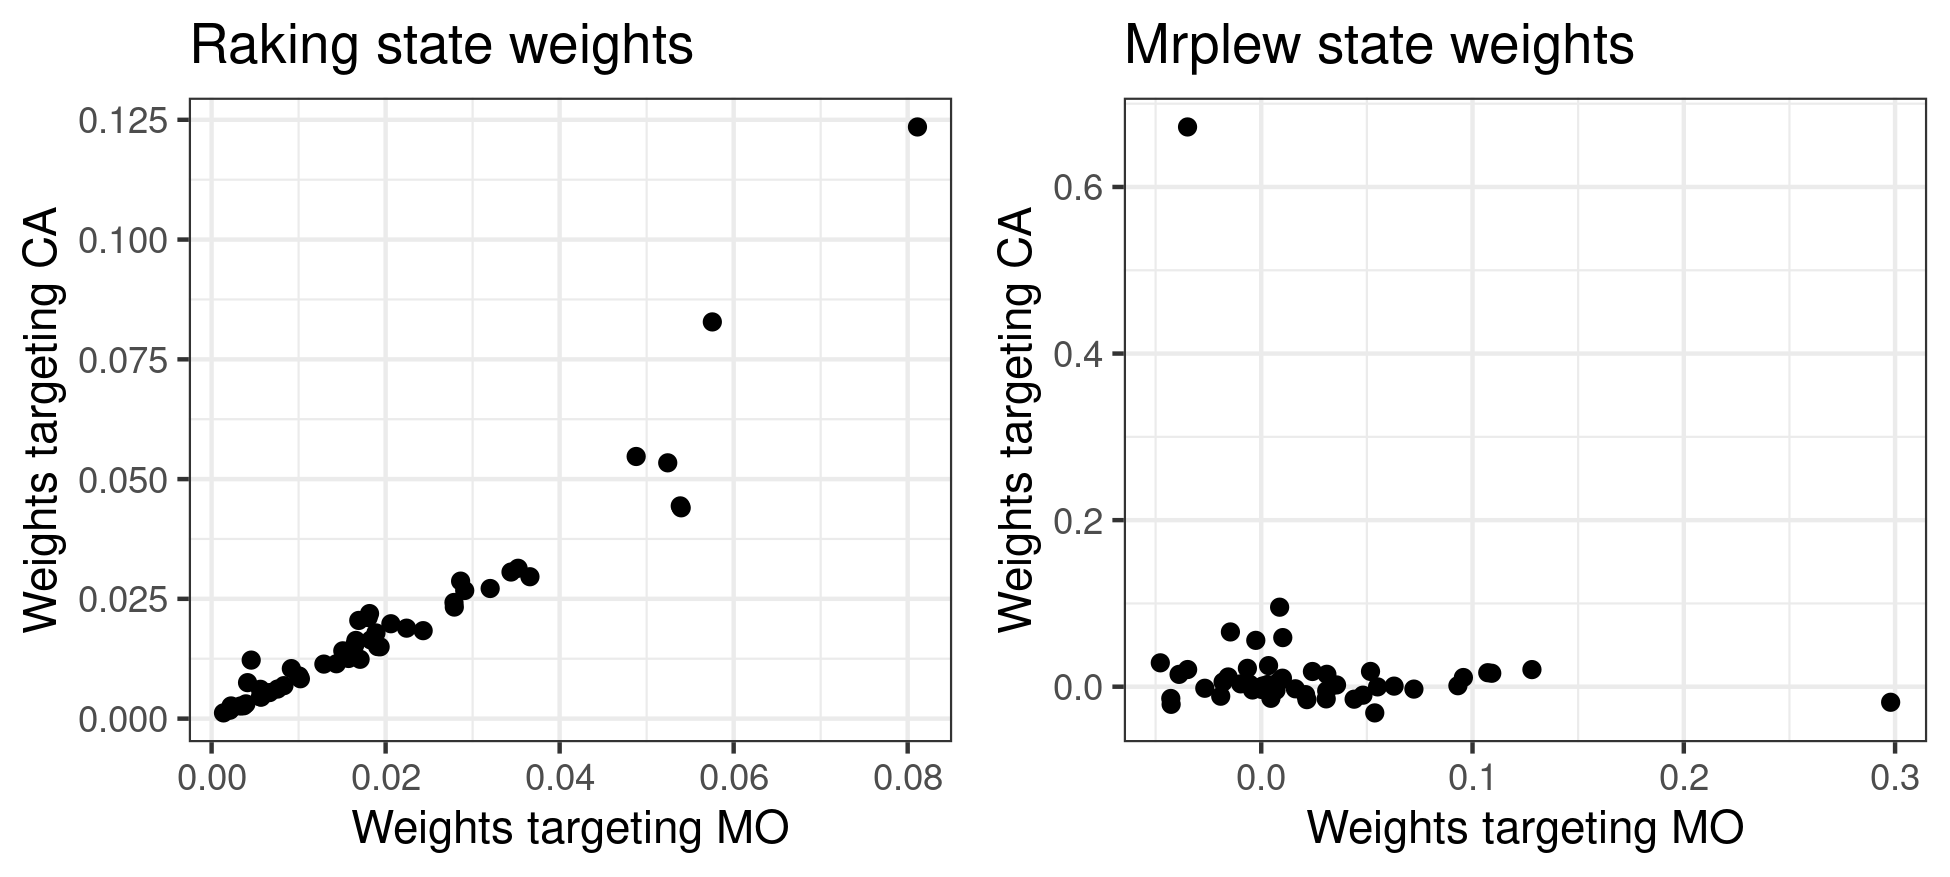
\includegraphics[width=0.98\linewidth,height=0.441\linewidth]{figure/poolingcompplot-1} 

}

\caption[]{Different variability in per-state subgroup contribution weights for Same-Sex Marriage. Each point is a state.}\label{fig:poolingcompplot}
\end{figure}

\end{knitrout}
}



\newcommand{\ImportanceSamplingPlot}{

\begin{knitrout}
\definecolor{shadecolor}{rgb}{0.969, 0.969, 0.969}\color{fgcolor}\begin{figure}[H]

{\centering 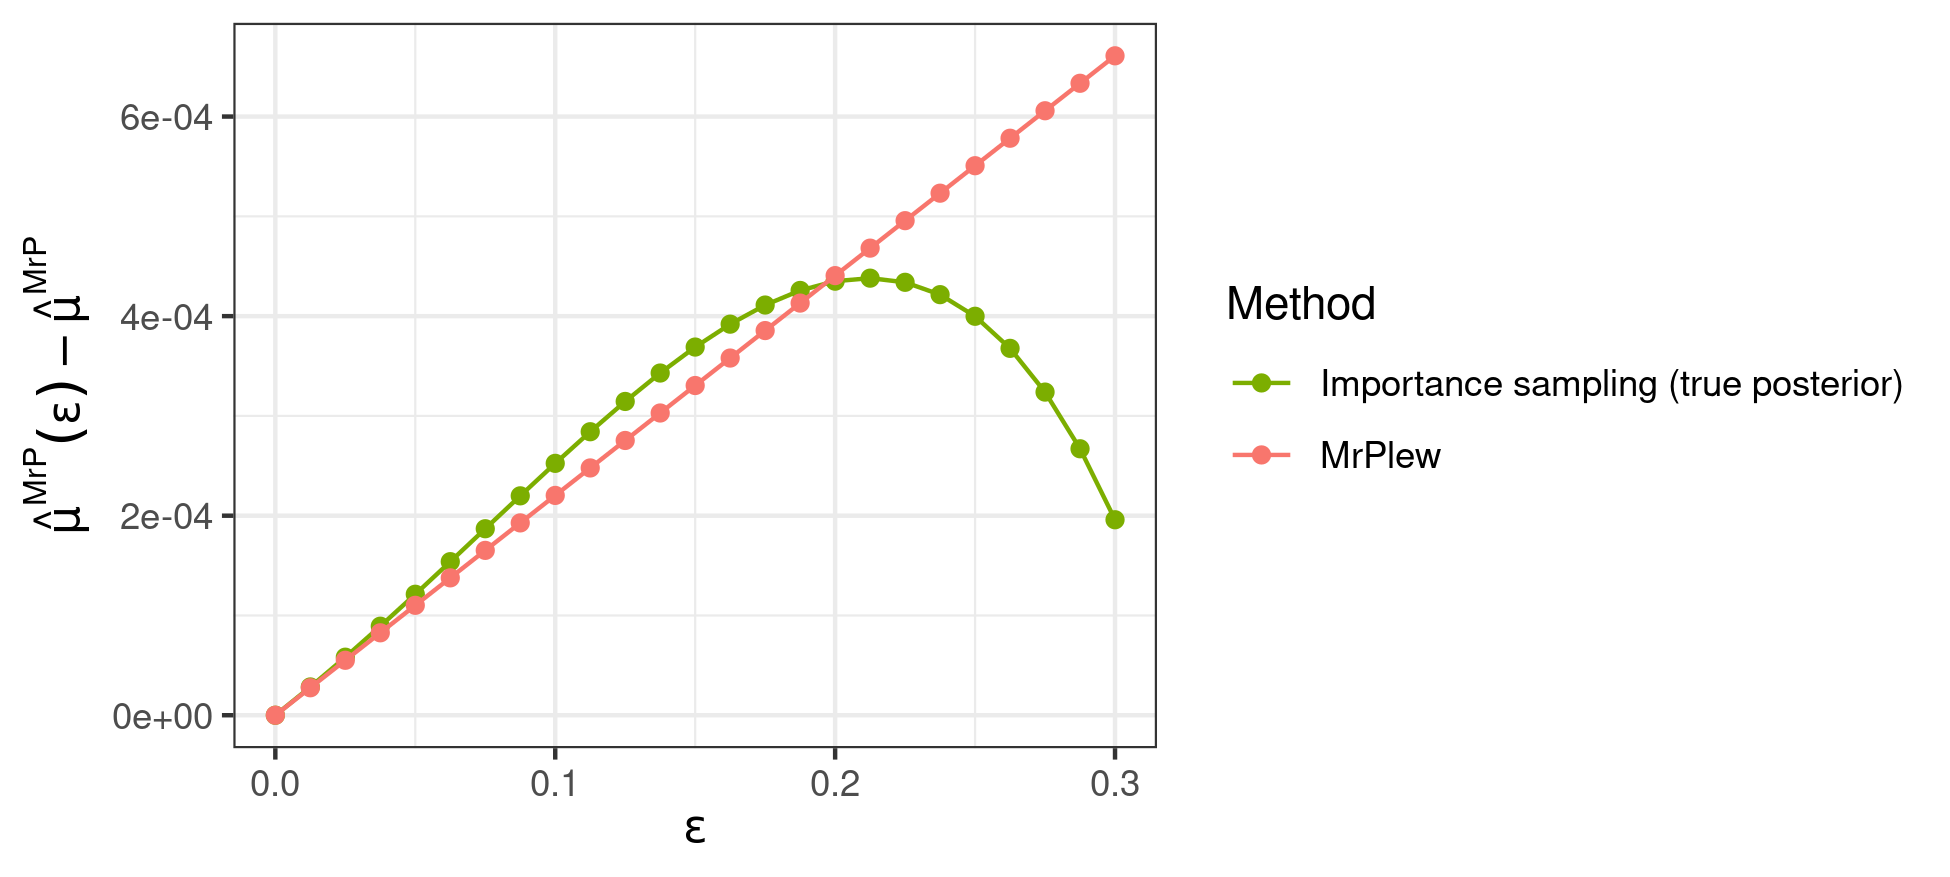
\includegraphics[width=0.98\linewidth,height=0.441\linewidth]{figure/isplot-1} 

}

\caption[]{Local behavior of the Same-Sex Marriage perturbation.  We only consider $\epsilon$ with at least 1000 effective self-normalized importance samples.}\label{fig:isplot}
\end{figure}

\end{knitrout}
}



\newcommand{\AlexanderModelsBalancePlot}{

\begin{knitrout}
\definecolor{shadecolor}{rgb}{0.969, 0.969, 0.969}\color{fgcolor}\begin{figure}[H]

{\centering 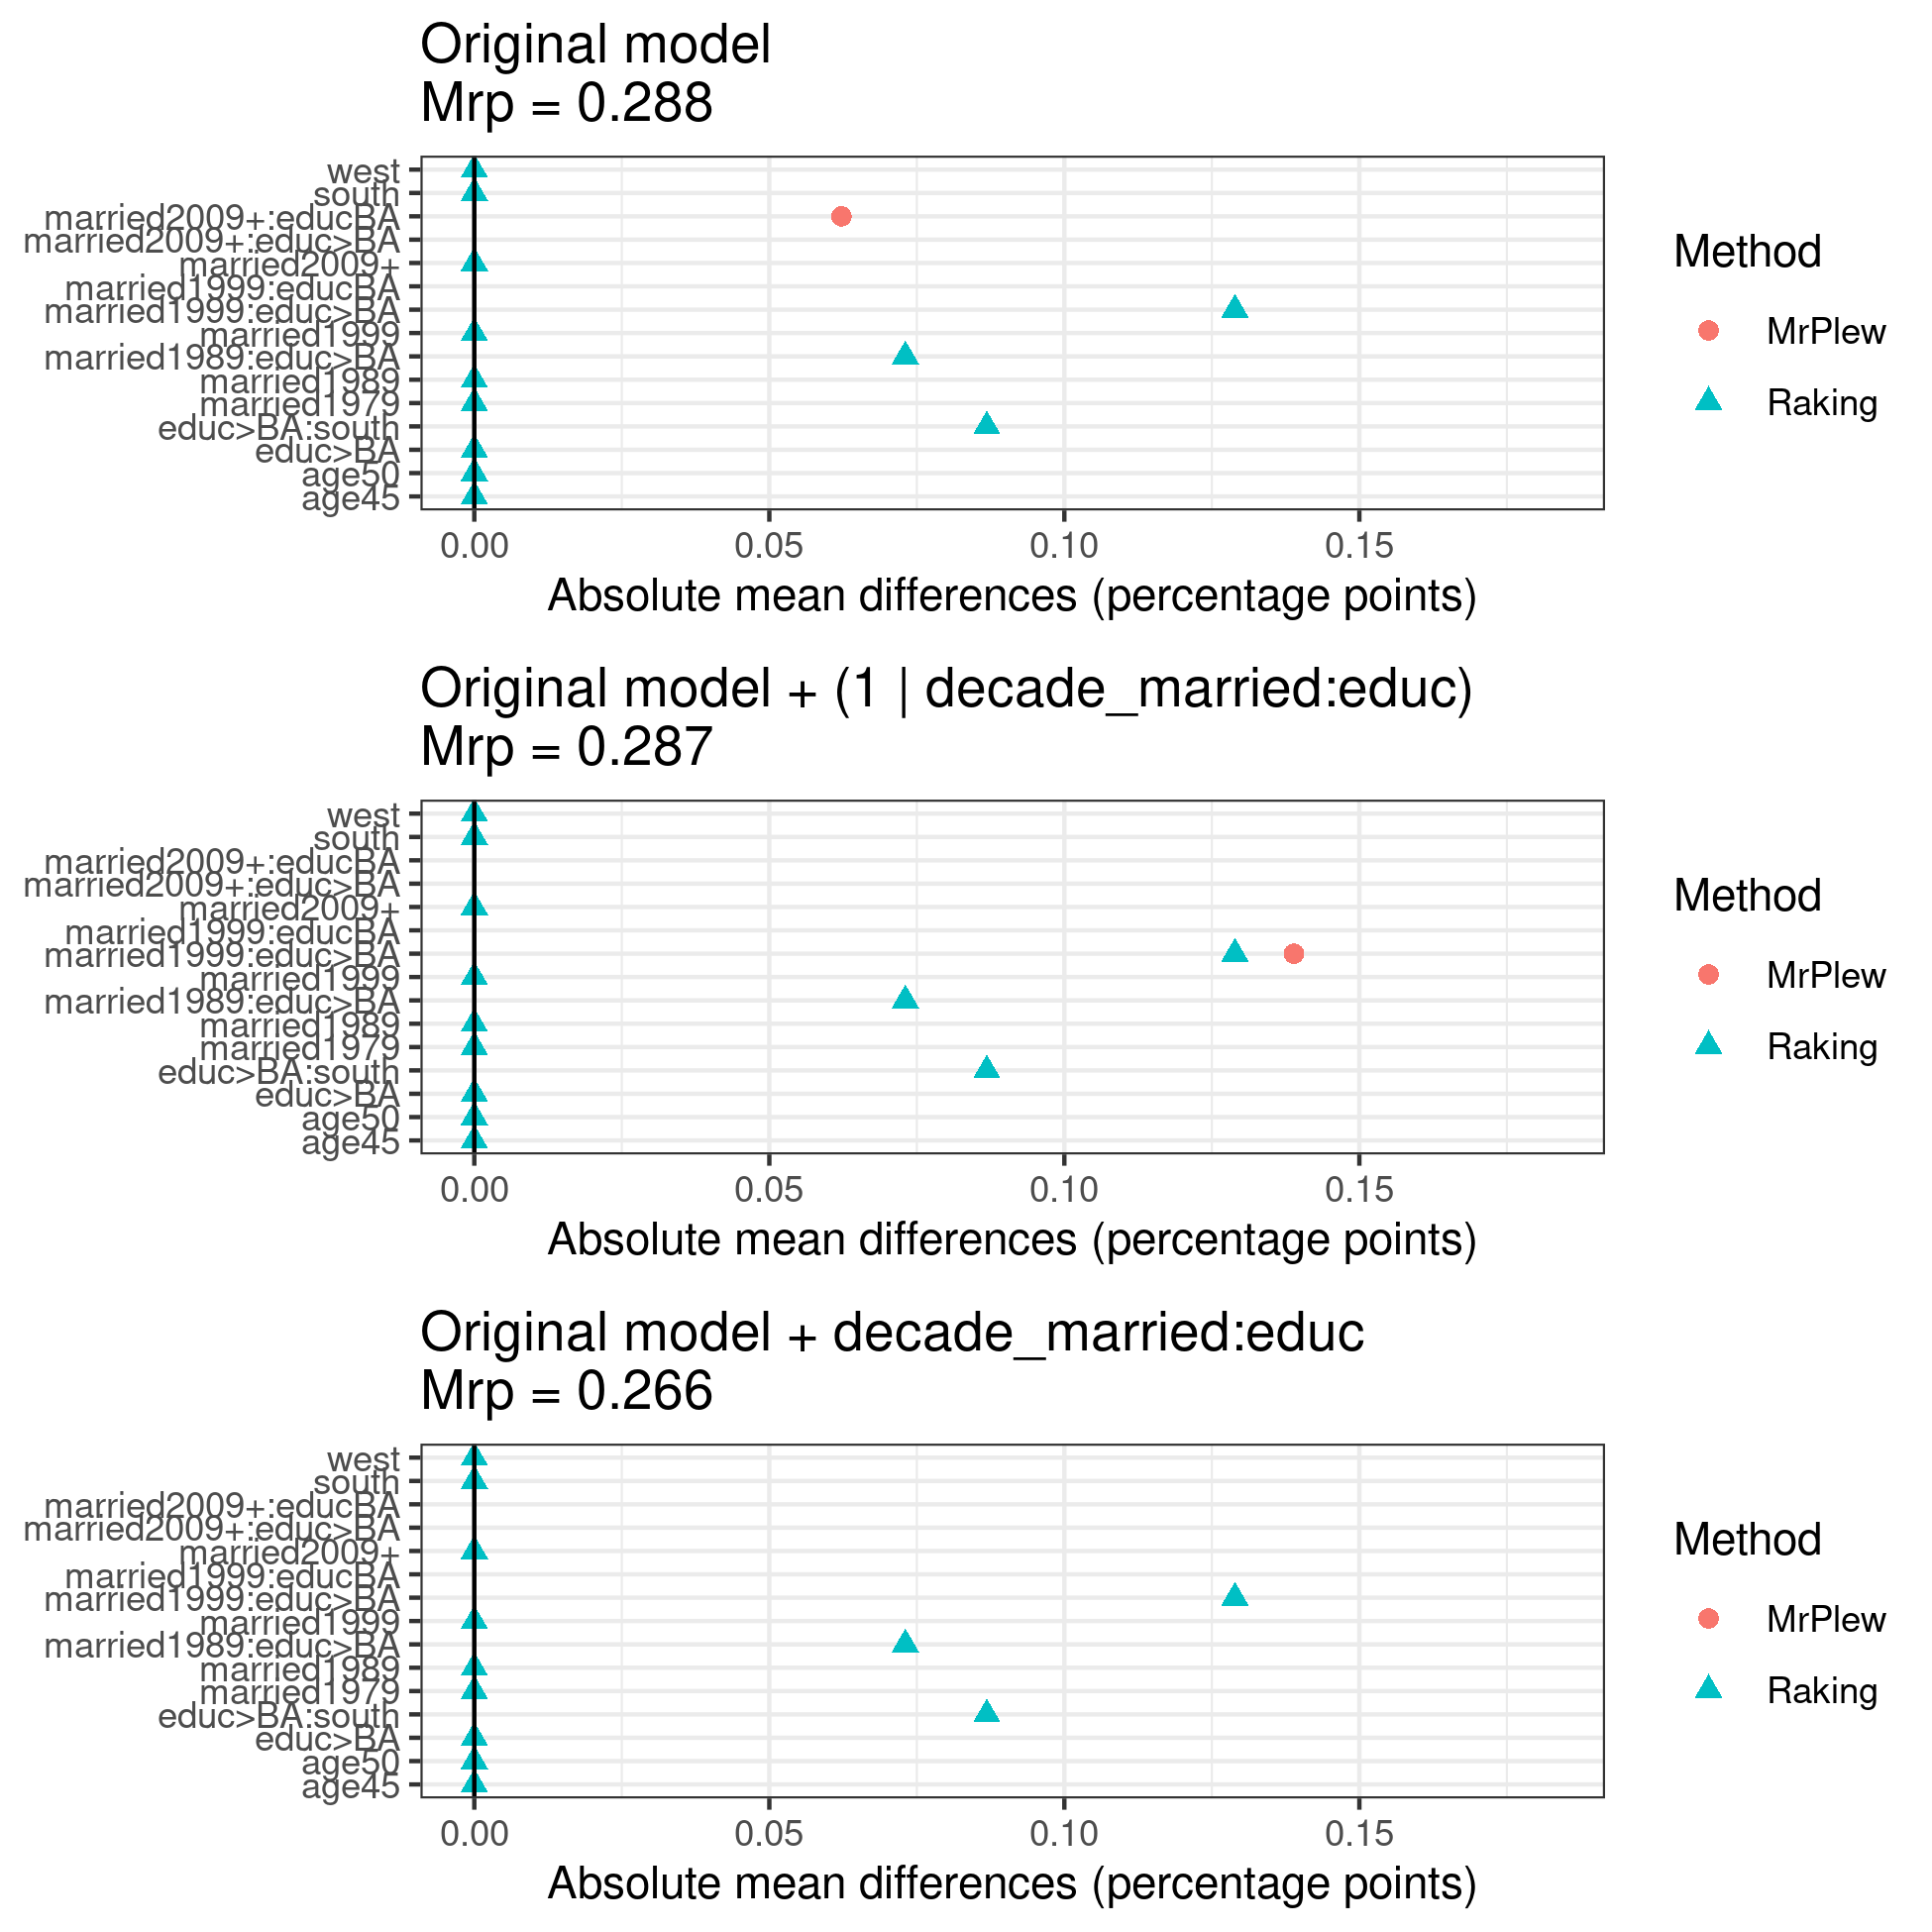
\includegraphics[width=0.98\linewidth,height=0.980\linewidth]{figure/alexandermodelsbalance-1} 

}

\caption[]{The effect of adding random and fixed effects for an imbalanced interaction in the Name Change analysis.  Any regressor showing an imbalance in any of the models above a certain threshold is shown in each plot, so regressors that are not shown can be assumed to be reasonably balanced.}\label{fig:alexandermodelsbalance}
\end{figure}

\end{knitrout}

}



